\documentclass[twocolumn,10pt]{article}

\usepackage{fontspec}

\usepackage{xunicode, xltxtra}

\usepackage{etoolbox}

\newbool{en}
\setbool{en}{false}

\newbool{cn}
\setbool{cn}{true}

\newtoggle{encn}
\settoggle{encn}{false}
 
%% \usepackage[slantfont,boldfont]{xeCJK}
\usepackage[PunctStyle=CCT]{xeCJK}

\setlength\textwidth{6.875in}
\setlength\textheight{8.875in}
% set both margins to 2.5 pc
\setlength{\oddsidemargin}{-0.1875in}% 1 - (8.5 - 6.875)/2
\setlength{\evensidemargin}{-0.1875in}
\setlength{\marginparwidth}{0pc}
\setlength{\marginparsep}{0pc}%
\setlength{\topmargin}{0in} \setlength{\headheight}{0pt}
\setlength{\headsep}{0pt}
\setlength{\footskip}{37pt}%
%\setlength{\columnsep}{0.3125in}
%\setlength{\columnwidth}{3.28125in}% (6.875 - 0.3125)/2 = 3.28125in
\setlength{\parindent}{1pc}
\newcommand{\myMargin}{1.00in}
\usepackage[top=\myMargin, left=\myMargin, right=\myMargin, bottom=\myMargin, nohead]{geometry}
\usepackage{epsfig,graphicx}
\usepackage{palatino}
\usepackage{fancybox}
\usepackage{url}
\usepackage[procnames]{listings}

% "define" Scala
\usepackage[T1]{fontenc}  
\usepackage[scaled=0.82]{beramono}  
\usepackage{microtype} 

\sbox0{\small\ttfamily A}
\edef\mybasewidth{\the\wd0 }

\lstdefinelanguage{scala}{
  morekeywords={abstract,case,catch,class,def,%
    do,else,extends,false,final,finally,%
    for,if,implicit,import,match,mixin,%
    new,null,object,override,package,%
    private,protected,requires,return,sealed,%
    super,this,throw,trait,true,try,%
    type,val,var,while,with,yield},
  sensitive=true,
  morecomment=[l]{//},
  morecomment=[n]{/*}{*/},
  morestring=[b]",
  morestring=[b]',
  morestring=[b]"""
}

\usepackage{color}
\definecolor{dkgreen}{rgb}{0,0.6,0}
\definecolor{gray}{rgb}{0.5,0.5,0.5}
\definecolor{mauve}{rgb}{0.58,0,0.82}

% Default settings for code listings
\lstset{frame=tb,
  language=scala,
  aboveskip=3mm,
  belowskip=3mm,
  showstringspaces=false,
  columns=fixed, % basewidth=\mybasewidth,
  basicstyle={\small\ttfamily},
  numbers=none,
  numberstyle=\footnotesize\color{gray},
  % identifierstyle=\color{red},
  keywordstyle=\color{blue},
  commentstyle=\color{dkgreen},
  stringstyle=\color{mauve},
  frame=single,
  breaklines=true,
  breakatwhitespace=true,
  procnamekeys={def, val, var, class, trait, object, extends},
  procnamestyle=\ttfamily\color{red},
  tabsize=2
}

\lstnewenvironment{scala}[1][]
{\lstset{language=scala,#1}}
{}
\lstnewenvironment{cpp}[1][]
{\lstset{language=C++,#1}}
{}
\lstnewenvironment{bash}[1][]
{\lstset{language=bash,#1}}
{}
\lstnewenvironment{verilog}[1][]
{\lstset{language=verilog,#1}}
{}



\lstset{frame=, basicstyle={\footnotesize\ttfamily}}

\newcommand{\todo}[1]{\emph{TODO: #1}}
\newcommand{\comment}[1]{\emph{Comment: #1}}

% uncomment following for final submission
\renewcommand{\todo}[1]{}
\renewcommand{\comment}[1]{}

\newenvironment{commentary}
{ \vspace{-0.1in}
  \begin{quotation}
  \noindent
  \small \em
  \rule{\linewidth}{1pt}\\
}
{
  \end{quotation}
}

% \newenvironment{kode}%
% {\footnotesize
%  %\setlength{\parskip}{0pt}
%   %\setlength{\topsep}{0pt}
%   %\setlength{\partopsep}{0pt}
%  \verbatim}
% {\endverbatim 
% %\vspace*{-0.1in}
%  }

% \newenvironment{kode}%
% {\VerbatimEnvironment
% \footnotesize\begin{Sbox}\begin{minipage}{6in}\begin{Verbatim}}%
% {\end{Verbatim}\end{minipage}\end{Sbox}
% \setlength{\fboxsep}{8pt}\fbox{\TheSbox}}

% \newenvironment{kode}
% {\begin{Sbox}
% \footnotesize
% \begin{minipage}{6in}
%   %\setlength{\parskip}{0pt}
%   %\setlength{\topsep}{0pt}
%   %\setlength{\partopsep}{0pt}
%   \verbatim}
% {\endverbatim 
% \end{minipage}
% \end{Sbox} 
% \fbox{\TheSbox}
%  %\vspace*{-0.1in}
%  }

\title{Chisel 3.0 Tutorial (Beta)}
\author{Jonathan Bachrach, Krste Asanovi\'{c}, John Wawrzynek \\
EECS Department, UC Berkeley\\
{\tt  \{jrb|krste|johnw\}@eecs.berkeley.edu} \\ \\
Translator: Sand River \\
{\tt  liwei.ma@gmail.com}
}
\date{\today}

\newenvironment{example}{\VerbatimEnvironment\begin{footnotesize}\begin{Verbatim}}{\end{Verbatim}\end{footnotesize}}
\newcommand{\kode}[1]{\begin{footnotesize}{\tt #1}\end{footnotesize}}

\def\code#1{{\tt #1}}

\def\note#1{\noindent{\bf [Note: #1]}}
%\def\note#1{}

\linespread{1.15}

\begin{document}
\maketitle{}

% TODO: default
% TODO: enum yields Bits
% TODO: why hardware construction languages
\ifbool{en}{\section{Introduction}}
\ifbool{cn}{\section{引言}}

\ifbool{en}{  
This document is a tutorial introduction to {\em Chisel} (Constructing
Hardware In a Scala Embedded Language).  Chisel is a hardware
construction language embedded in the high-level programming language
Scala.  At some point we will provide a proper reference manual, in
addition to more tutorial examples.  In the meantime, this document
along with a lot of trial and error should set you on your way to
using Chisel.  Chisel is really only a set of special class
definitions, predefined objects, and usage conventions within Scala,
so when you write a Chisel program you are actually writing a Scala
program.  However, for the tutorial we don't presume that you
understand how to program in Scala.  We will point out necessary Scala
features through the Chisel examples we give, and significant hardware
designs can be completed using only the material contained herein.
But as you gain experience and want to make your code simpler or more
reusable, you will find it important to leverage the underlying power
of the Scala language. We recommend you consult one of the excellent
Scala books to become more expert in Scala programming.
}
\ifbool{cn}{
本文档是{\em Chisel} (Constructing Hardware In a Scala Embedded Language) 的介绍性教程。
Chisel是一种嵌入在高阶编程语言Scala中用来构造硬件的语言。
在未来的某个时候我们将提供更适合的参考手册,引入更多的教程示例。
在这之前,本文档虽然有一些尝试和错误,但也应该可以带你开始使用Chisel。
Chisel实际上只是一组特殊的用Scala事先定义的类、对象和使用惯例,所以当写一份Chisel程序的时候,你实际上在写一份Scala程序。
我们会在讲述我们的Chisel示例的时候指明必要的Scala语法特性,根据本文档给出的材料应该就可以完成相当有意义的硬件设计。
但是如果你还想体验和设计出简洁和高复用的代码,你会发现借用Scala语言潜在的优势非常重要。
我们建议你翻阅一些优秀的Scala书籍以便在使用Scala编程的时候更加专业。
}


\ifbool{en}{
% MS: maybe infancy can now be dropped. Chisel has proven
% to be mature enough for serious designs.
Chisel is still in its infancy and you are likely to encounter some
implementation bugs, and perhaps even a few conceptual design
problems.  However, we are actively fixing and improving the language,
and are open to bug reports and suggestions.  Even in its early state,
we hope Chisel will help designers be more productive in building
designs that are easy to reuse and maintain.
}
\ifbool{cn}{%%%%%%%%%%%%%%%%%%%%%%%%%%%%%%%%%%%%%%%%
Chisel现在还处于早期阶段,你有可能会遇到一些实现缺陷,甚至有可能遇到方案设计问题。
然而我们正在积极的修正和改进这种语言,欢迎提交缺陷报告和改进建议。
即使在它的早期阶段,我们希望Chisel可以帮助设计者在构建容易复用和维护的设计中提高生产力。
}%%%%%%%%%%%%%%%%%%%%%%%%%%%%%%%%%%%%%%%%%


\begin{commentary}
\ifbool{en}{
Through the tutorial, we format commentary on our design choices as in
this paragraph.  You should be able to skip the commentary sections
and still fully understand how to use Chisel, but we hope you'll find
them interesting.
}
\ifbool{cn}{
在本教程中这样版式的段落里,我们评述设计该语言时的各种选择。
你可以跳过这些评述章节而完全不会影响理解如何使用Chisel,但是我们希望你能发现这些章节的有趣之处。
}


\ifbool{en}{
We were motivated to develop a new hardware language by years of
struggle with existing hardware description languages in our research
projects and hardware design courses.  Verilog and VHDL were developed
as hardware {\em simulation} languages, and only later did they become
a basis for hardware {\em synthesis}.  Much of the semantics of these
languages are not appropriate for hardware synthesis and, in fact,
many constructs are simply not synthesizable.  Other constructs are
non-intuitive in how they map to hardware implementations, or their
use can accidently lead to highly inefficient hardware structures.
While it is possible to use a subset of these languages and yield
acceptable results, they nonetheless present a cluttered and confusing
specification model, particularly in an instructional setting.
}
\ifbool{cn}{
在数年的研究项目和硬件教学实践中一直和现有的硬件描述语言做斗争,我们非常有一种开发新的硬件语言的冲动。
Verilog和VHDL在设计之初只是硬件{\bf 模拟}语言,仅仅在后来才成为硬件{\bf 综合}的基石。
这些语言的很多语法都不适合硬件综合,实际上很多语法概念完全不是可综合的。
另一些语法概念在如何映射到硬件实现方面是非常不直观的,或者一不小心就会导致非常低效的电路结构。
使用这些语言的一个子集生成合意的结果未尝不可,然而它们表达的规范模型毕竟是杂乱和混淆的,在教学过程中这些现象尤其明显。
}


\ifbool{en}{
However, our strongest motivation for developing a new hardware
language is our desire to change the way that electronic system design
takes place.  We believe that it is important to not only teach
students how to design circuits, but also to teach them how to design
{\em circuit generators}---programs that automatically generate
designs from a high-level set of design parameters and constraints.
Through circuit generators, we hope to leverage the hard work of
design experts and raise the level of design abstraction for everyone.
To express flexible and scalable circuit construction, circuit
generators must employ sophisticated programming techniques to make
decisions concerning how to best customize their output circuits
according to high-level parameter values and constraints.  While
Verilog and VHDL include some primitive constructs for programmatic
circuit generation, they lack the powerful facilities present in
modern programming languages, such as object-oriented programming,
type inference, support for functional programming, and reflection.
}
\ifbool{cn}{
而且,我们开发新的硬件语言的强烈冲动来自于我们对改变现有的电子系统的设计方法的渴望。
我们坚信,教会学生如何设计电路固然重要,更加重要的是教会他们如何设计{\bf 电路生成器} --- 能够根据一组高阶的设计参数和约束自动生成电路的程序。
通过电路生成器,我们期望可以借用设计专家的才干提升每个工程师的设计抽象水平。
为了表达灵活而可扩展的电路构造,电路生成器必须利用精致的编程技巧,在考虑如何更好的定制产生的电路的时候就可以做出更好的设计选择,以满足高阶的参数值和限制条件。
虽然Verilog和VHDL也包括了一些构造原语可以实现电路的程序化生成,但还是缺少现代编程语言中的强大的设施,诸如面向对象的编程,类型推断,函数式编程和反省机制。
}


\ifbool{en}{
Instead of building a new hardware design language from scratch, we
chose to embed hardware construction primitives within an existing
language.  We picked Scala not only because it includes the
programming features we feel are important for building circuit
generators, but because it was specifically developed as a base for
domain-specific languages.
}
\ifbool{cn}{
我们选择把硬件构造原语嵌入在一个现有的语言中,而不是从头构建一个新的硬件设计语言。
我们选择Scala不仅因为它包括了一些编程特性,我们认为对构造电路生成器非常重要,而且因为它是专门为成为领域专用语言的基础而开发的。
}

\end{commentary}

\ifbool{en}{
\section{Hardware expressible in Chisel}
}
\ifbool{cn}{
\section{Chisel可表达的硬件}
}

% The initial version of Chisel only supports the expression of
% synchronous RTL (Register-Transfer Level) designs, with a single
% common clock.  Synchronous RTL circuits can be expressed as a
% hierarchical composition of modules containing combinational logic and
% clocked state elements.  Although Chisel assumes a single global
% clock, local clock gating logic is automatically generated for every
% state element in the design to save power.
% \begin{commentary}
% Modern hardware designs often include multiple islands of logic, where
% each island uses a different clock and where islands must correctly
% communicate across clock island boundaries.  Although clock-crossing
% synchronization circuits are notoriously difficult to design, there
% are known good solutions for most scenarios, which can be packaged as
% library elements for use by designers.  As a result, most effort in
% new designs is spent in developing and verifying the functionality
% within each synchronous island rather than on passing values between
% islands.
% 
% In its current form, Chisel can be used to describe each of the
% synchronous islands individually. Existing tool frameworks can tie
% together these islands into a complete design.  For example, a
% separate outer simulation framework can be used to model the assembly
% of islands running together.  It should be noted that exhaustive
% dynamic verification of asynchronous communications is usually
% impossible and that more formal static approaches are usually
% necessary.
% \end{commentary}
\ifbool{en}{
This version of Chisel only supports binary logic, and does not
support tri-state signals.
}
\ifbool{cn}{
本版本的Chisel只支持二值逻辑,不支持三态信号。
}

\begin{commentary}
\ifbool{en}{
We focus on binary logic designs as they constitute the vast majority
of designs in practice.  We omit support for tri-state logic in the
current Chisel language as this is in any case poorly supported by
industry flows, and difficult to use reliably outside of controlled
hard macros.
}
\ifbool{cn}{
我们聚焦在二值逻辑设计是因为其囊括实际应用中绝大部分的设计。
在当前Chisel语言中我们省略了三态逻辑的支持,因为无论如何它在工业流程中的支持都很差劲,在受控的硬件宏块外也很难被可靠的使用。
}

\end{commentary}

\ifbool{en}{
\section{Datatypes in Chisel}
}
\ifbool{cn}{
\section{Chisel的数据类型}
}

\ifbool{en}{
Chisel datatypes are used to specify the type of values held in state
elements or flowing on wires.  While hardware designs ultimately
operate on vectors of binary digits, other more abstract
representations for values allow clearer specifications and help the
tools generate more optimal circuits.  In Chisel, a raw collection of
bits is represented by the \code{Bits} type.  Signed and unsigned integers
are considered subsets of fixed-point numbers and are represented by
types \code{SInt} and \code{UInt} respectively. Signed fixed-point
numbers, including integers, are represented using two's-complement
format.  Boolean values are represented as type \code{Bool}.  Note
that these types are distinct from Scala's builtin types such as
\code{Int} or \code{Boolean}.  Additionally, Chisel defines {\em Bundles} for making
collections of values with named fields (similar to {\em structs} in
other languages), and {\em Vecs} for indexable collections of
values.  Bundles and Vecs will be covered later.
}
\ifbool{cn}{
Chisel的数据类型用来表明在状态单元上保存或者信号线上流动的数值的类型。
虽然硬件设计最终都是在操作二值数码的向量,然而更抽象的数值表示方法容许定义更清晰的规范,帮助工具生成更加优化的电路。
在Chisel中,\code{Bits} 类型表示多个比特的简单集合。
有符号和无符号整数是定点数字的子集,分别用\code{SInt}类型和\code{UInt}类型表示。
有符号定点数字,包括整数,使用二进制补码形式表示。
布尔数值用\code{Bool}类型表示。
请注意这些类型明显区别于Scala 内建的类型,比如\code{Int}和\code{Boolean}。
}


\ifbool{en}{
Constant or literal values are expressed using Scala integers or
strings passed to constructors for the types:
}
\ifbool{cn}{
常量和字面数值表示成Scala整数或者附有对应类型构造器的字符串:
}

\begin{scala}
1.U       // decimal 1-bit lit from Scala Int.
"ha".U    // hexadecimal 4-bit lit from string.
"o12".U   // octal 4-bit lit from string.
"b1010".U // binary 4-bit lit from string.

5.S    // signed decimal 4-bit lit from Scala Int.
-8.S   // negative decimal 4-bit lit from Scala Int.
5.U    // unsigned decimal 3-bit lit from Scala Int.

true.B // Bool lits from Scala lits.
false.B
\end{scala}


\ifbool{en}{
By default, the Chisel compiler will size each constant to the minimum
number of bits required to hold the constant, including a sign bit for
signed types.  Bit widths can also be specified explicitly on
literals, as shown below:
}
\ifbool{cn} {
Chisel编译器默认使用最小的位宽来保存常量,有符号类型会包括一个符号比特。
字面数字也可以显式地指明位宽,如下所示:
}


\begin{scala}
"ha".U(8.W)     // hexadecimal 8-bit lit of type UInt
"o12".U(6.W)    // octal 6-bit lit of type UInt
"b1010".U(12.W) // binary 12-bit lit of type UInt

5.S(7.W) // signed decimal 7-bit lit of type SInt
5.U(8.W) // unsigned decimal 8-bit lit of type UInt
\end{scala}

\ifbool{en}{
\noindent
For literals of type \code{UInt}, the value is
zero-extended to the desired bit width.  For literals of type
\code{SInt}, the value is sign-extended to fill the desired bit width.
If the given bit width is too small to hold the argument value, then a
Chisel error is generated.
}
\ifbool{cn}{
\noindent
\code{UInt}类型的字面常量的数值用零扩展到目标位宽。
\code{SInt}类型的字面常量的数值用符号为扩展到目标位宽。
如果给出的位宽太小不能保存参量数值,Chisel会报错。
}

\begin{commentary}
\ifbool{en}{
We are working on a more concise literal syntax for Chisel using
symbolic prefix operators, but are stymied by the limitations of Scala
operator overloading and have not yet settled on a syntax that is
actually more readable than constructors taking strings.

We have also considered allowing Scala literals to be automatically
converted to Chisel types, but this can cause type ambiguity and
requires an additional import.

The SInt and UInt types will also later support an optional exponent
field to allow Chisel to automatically produce optimized fixed-point
arithmetic circuits.
}
\ifbool{cn}{
%% 我们正在试图使用符号化的前缀操作符构建更精确的Chisel字面常量的语法,但是受阻于Scala操作符重载的限制,还没有能够实现更可读的语法,现在只能使用字符串来构造。
我们正在想办法设计更精确的Chisel字面常量的语法,比如使用符号化的前缀操作符。但是受阻于Scala操作符重载的限制,理想的更可读的语法还没能实现,现在只能使用字符串构造字面常量。

我们也考虑过允许Scala字面常量自动的转换到Chisel类型,但这会导致含混的语法,需要追加额外的导入。

\code{SInt}和\code{UInt}类型以后会支持可选的指数域,这样Chisel就可以自动的产生优化的定点算术电路。
}

\end{commentary}

\ifbool{en}{
\section{Combinational Circuits}
}
\ifbool{cn}{
\section{组合电路}
}

\ifbool{en}{
A circuit is represented as a graph of nodes in Chisel.  Each node is
a hardware operator that has zero or more inputs and that drives one
output.  A literal, introduced above, is a degenerate kind of node
that has no inputs and drives a constant value on its output.  One way
to create and wire together nodes is using textual expressions.  For
example, we can express a simple combinational logic circuit
using the following expression:
}
\ifbool{cn}{
电路在Chisel中表示成节点间的图。
每个节点是一个硬件操作符,拥有零个或多个输入,驱动一个输出。
前面所述的字面常量是退化的节点,没有输入,输出一个常量。
一种常见的创建和连接节点方法便是使用文本表达式。
例如,使用下面的表达式我们可以表达一个简单的组合逻辑电路:
}


\begin{scala}
(a & b) | (~c & d)
\end{scala}

\ifbool{en}{
The syntax should look familiar, with \code{\&} and \code{|}
representing bitwise-AND and -OR respectively, and \code{\~{}}
representing bitwise-NOT.  The names \code{a} through \code{d}
represent named wires of some (unspecified) width.

Any simple expression can be converted directly into a circuit tree,
with named wires at the leaves and operators forming the internal
nodes.  The final circuit output of the expression is taken from the
operator at the root of the tree, in this example, the bitwise-OR.

Simple expressions can build circuits in the shape of trees, but to
construct circuits in the shape of arbitrary directed acyclic graphs
(DAGs), we need to describe fan-out.  In Chisel, we do this by naming
a wire that holds a subexpression that we can then reference multiple
times in subsequent expressions.  We name a wire in Chisel by
declaring a variable.  For example, consider the select expression,
which is used twice in the following multiplexer description:
}
\ifbool{cn}{
这些语法看起来应该很熟悉,\code{\&} 表示按位与,\code{|} 表示按位或,\code{\~{}} 表示按位非。
从\code{a}到\code{d}的这些名称表示一定位宽(尚未指明)的有确定名称的信号线。

任何简单的表达式都可以直接转换成一个树状电路,命了名的信号线是叶子,操作符是内部节点。
在树的根节点操作符上获得表达式最终电路的输出,这个操作符在本例中就是那个位或。

简单的表达式可以构造树形的电路,但是为了构造任意有向无环图(DAG)形状的电路,我们必须能够描述电路扇出。
在Chisel中,为了实现扇出,我们可以用命名的信号线来捕获一个子表达式,然后在后续的表达式中多次引用这个信号线。
在Chisel中,我们通过声明一个变量来命名一个信号线。
例如,在下面这个多路选择描述中,这个选择表达式被使用了两次:
}


\begin{scala}
val sel = a | b
val out = (sel & in1) | (~sel & in0)
\end{scala}

\ifbool{en}{
\noindent
The keyword \code{val} is part of Scala, and is used to name variables
that have values that won't change.  It is used here to name the
Chisel wire, \code{sel}, holding the output of the first bitwise-OR
operator so that the output can be used multiple times in the second
expression.
}
\ifbool{cn}{
\noindent
关键字\code{val}来源于Scala,是给那些值不更改的变量命名的。
这里被用来给Chisel的信号线命名,信号线\code{sel}捕获了第一个位或操作符的输出,便可以在第二个表达式中重复使用它。 
}

\ifbool{en}{
\section{Builtin Operators}
}
\ifbool{cn}{
\section{内建操作符}
}

\ifbool{en}{
Chisel defines a set of hardware operators for the builtin types shown
in Table~\ref{tbl:chisel-operators}.
}
\ifbool{cn}{
Chisel为内建数据类型定义了硬件操作符,如表~\ref{tbl:chisel-operators} 所示。
}


\begin{table*}
\begin{center}
\begin{tabular}{|l|l|}
\hline
Example & Explanation \\
\hline
\hline
\multicolumn{2}{|l|}{Bitwise operators.  Valid on SInt, UInt, Bool.} \\
\hline
\hline
\verb!val invertedX = ~x!                    &   Bitwise NOT  \\
\verb!val hiBits = x & "h_ffff_0000".U ! &   Bitwise AND  \\
\verb!val flagsOut = flagsIn | overflow !    &   Bitwise OR   \\
\verb!val flagsOut = flagsIn ^ toggle !      &   Bitwise XOR  \\
\hline
\hline
\multicolumn{2}{|l|}{Bitwise reductions.  Valid on SInt and
  UInt.  Returns Bool. } \\
\hline
\hline
\verb!val allSet = andR(x) ! & AND reduction  \\
\verb!val anySet = orR(x)  ! & OR reduction   \\
\verb!val parity = xorR(x) !  & XOR reduction  \\
\hline
\hline
\multicolumn{2}{|l|}{Equality comparison. Valid on SInt, 
UInt, and Bool. Returns Bool.} \\
\hline
\hline
\verb@val equ = x === y@ & Equality \\
\verb@val neq = x =/= y@ & Inequality \\
\hline
\hline
\multicolumn{2}{|l|}{Shifts. Valid on SInt and UInt.} \\
\hline
\hline
\verb@val twoToTheX = 1.S << x@  & Logical left shift. \\
\verb@val hiBits = x >> 16.U@          & Right shift (logical on UInt and\&
arithmetic on SInt). \\
% \verb@val scaledX = x >>> 3@  & Arithmetic right shift, copies in sign bits. \\
\hline
\hline
\multicolumn{2}{|l|}{Bitfield manipulation.  Valid on SInt, UInt, and Bool. } \\
\hline
\hline
\verb@val xLSB = x(0)@  & Extract single bit, LSB has index 0. \\
\verb@val xTopNibble = x(15,12)@  & Extract bit field  from end to start
bit position. \\
\verb@val usDebt = Fill(3, "hA".U)@ & Replicate a bit string multiple times. \\
\verb@val float = Cat(sign,exponent,mantissa)@ & Concatenates bit fields, with first argument on left.\\
\hline
\hline
\multicolumn{2}{|l|}{Logical operations.  Valid on Bools. } \\
\hline
\verb@val sleep = !busy@  & Logical NOT \\
\verb@val hit = tagMatch && valid @  & Logical AND \\
\verb@val stall = src1busy || src2busy@  & Logical OR \\
\verb@val out = Mux(sel, inTrue, inFalse)@  & Two-input mux where sel is a Bool \\ % {\bf Why?} \\
\hline
\hline
\multicolumn{2}{|l|}{Arithmetic operations.  Valid on Nums: SInt and UInt. } \\
\hline
\verb@val sum = a + b@  & Addition \\
\verb@val diff = a - b @  & Subtraction \\
\verb@val prod = a * b @  & Multiplication \\
\verb@val div = a / b @  & Division \\
\verb@val mod = a % b @  & Modulus \\
\hline
\hline
\multicolumn{2}{|l|}{Arithmetic comparisons.  Valid on Nums: SInt and
  UInt. Returns Bool.} \\
\hline
\verb@val gt = a > b@  & Greater than \\
\verb@val gte = a >= b@  & Greater than or equal \\
\verb@val lt = a < b@  & Less than \\
\verb@val lte = a <= b@  & Less than or equal \\
\hline
\end{tabular}
\end{center}
\caption{Chisel operators on builtin data types.}
\label{tbl:chisel-operators}
\end{table*}

\ifbool{en}{
\subsection{Bitwidth Inference}
}
\ifbool{cn}{
\subsection{位宽推断}
}

\ifbool{en}{
Users are required to set bitwidths of ports and registers, but otherwise,
bit widths on wires are automatically inferred unless set manually by the user.
% TODO: how do you set the width explicitly?
The bit-width inference engine starts from the graph's input ports and 
calculates node output bit widths from their respective input bit widths according to the following set of rules:
}
\ifbool{cn}{
用户需要为端口和寄存器设置位宽,然而信号线上的位宽也可以被自动的推断出来,除非已经被用户手工设置。
位宽推断引擎从图的输入端口开始,根据下面的规则集从节点相应的输入的位宽计算其输出的位宽。 
}


\begin{tabular}{ll}
{\bf operation} & {\bf bit width} \\ 
\verb|z = x + y| & \verb|wz = max(wx, wy)| \\
\verb+z = x - y+ & \verb|wz = max(wx, wy)|\\
\verb+z = x & y+ & \verb+wz = min(wx, wy)+ \\
\verb+z = Mux(c, x, y)+ & \verb+wz = max(wx, wy)+ \\
\verb+z = w * y+ & \verb!wz = wx + wy! \\
\verb+z = x << n+ & \verb!wz = wx + maxNum(n)! \\
\verb+z = x >> n+ & \verb+wz = wx - minNum(n)+ \\
\verb+z = Cat(x, y)+ & \verb!wz = wx + wy! \\
\verb+z = Fill(n, x)+ & \verb+wz = wx * maxNum(n)+ \\
% \verb+z = x < y+ & \verb+<= > >= && || != ===+ & \verb+wz = 1+ \\
\end{tabular}

\ifbool{en}{
\noindent
where for instance $wz$ is the bit width of wire $z$, and the \verb+&+
rule applies to all bitwise logical operations.
}
\ifbool{cn}{
这里以 $wz$ 为例,是信号线 $z$ 的位宽,并且 \code{\&} 操作的推断规则适用于所有的按位逻辑操作。
}

\comment{maxNum and MinNum need to be explained.}

\ifbool{en}{
The bit-width inference process continues until no bit width changes.
Except for right shifts by known constant amounts, the bit-width
inference rules specify output bit widths that are never smaller than
the input bit widths, and thus, output bit widths either grow or stay
the same.  Furthermore, the width of a register must be specified by
the user either explicitly or from the bitwidth of the reset value or
the \emph{next} parameter.
From these two requirements, we can show that the bit-width inference
process will converge to a fixpoint.
}
\ifbool{cn}{
位宽推断程序会一直进行到没有位宽再变化为止。
除非操作是右移已知的常量位宽,位宽推断规则规定输出的位宽永远不会小于输入的位宽,因此输出的位宽跟输入相比或者增加或者保持。
另外,用户必须显式地设置寄存器的位宽,或者指定为其复位数值的位宽,或者指定为其{\em 下一状态}的相关参数。
根据这两项规定,我们可以认定位宽推断程序最终会收敛到一个定点数。
}


\begin{commentary}
\ifbool{en}{
Our choice of operator names was constrained by the Scala language.
We have to use triple equals \code{===} for equality and \code{=/=}
for inequality to allow the
native Scala equals operator to remain usable.

We are also planning to add further operators that constrain bitwidth
to the larger of the two inputs.
}
\ifbool{cn}{
由于操作符名字的选择受限于Scala语言,我们不得不使用三个等号 \code{===} 来表示相等, 用 \code{=/=} 来表示不相等。
这样Scala原有的判断相等的操作符可以继续按原意使用。

我们也在考虑增加新的操作符,可以强迫输出位宽等于两个输入的较大的位宽。
}


\end{commentary}

\ifbool{en}{
\section{Functional Abstraction}
}
\ifbool{cn}{
\section{函数式抽象}
}

\ifbool{en}{
We can define functions to factor out a repeated piece of logic that
we later reuse multiple times in a design.  For example, we can wrap
up our earlier example of a simple combinational logic block as
follows:
}
\ifbool{cn}{
我们可以把重复使用的一段逻辑定义成函数,然后在一个设计中复用多次。
例如,我们可以把前面例子中的那个简单的组合逻辑块包装成如下的函数:
}


\begin{scala}
def clb(a: UInt, b: UInt, c: UInt, d: UInt): UInt = 
  (a & b) | (~c & d)
\end{scala}

\ifbool{en}{
\noindent
where \code{clb} is the function which takes \code{a}, \code{b},
\code{c}, \code{d} as arguments and returns a wire to the output of a
boolean circuit.  The \code{def} keyword is part of Scala and
introduces a function definition, with each argument followed by a colon then its type,
and the function return type given after the colon following the
argument list.  The equals (\code{=})
sign separates the function argument list from the function
definition.
}
\ifbool{cn}{
此处 \code{clb} 就是那个函数,它输入\code{a}, \code{b}, \code{c}, \code{d} 作为参数,返回一个信号线,这个信号线连接在一个布尔电路的输出信号上。
关键字 \code{def} 来自于Scala语言,用来定义一个函数。
在函数定义中,每个参数跟着它的数据类型,用冒号隔开,在参数列表的后面跟着函数的返回类型,同样也是用冒号隔开。
等号(\code{=})分隔开函数的参数列表和它的定义段落。
}


\ifbool{en}{
We can then use the block in another circuit as follows:
}
\ifbool{cn}{
这样我们就可以像这样在其他电路中使用这个函数块了:
}


\begin{scala}
val out = clb(a,b,c,d)
\end{scala}

% TODO: SHIFTER DONE FUNCTIONAL WITH LOOP

%% Because Scala has powerful type inference, we can in many cases drop
%% the type declarations on the function:
%% \begin{scala}
%% def clb(a, b, c, d) = (a & b) | (~c & d) // No types needed.

%% def bigblock(a: Bool, b: Bool, c: Bool, d: Bool,
%%              f: UInt, g: UInt, h: UInt, i: UInt): Bool =
%%                  clb(a, b, c, clb(f,g,h,i)!=0) 

%% \end{scala}

%% Here, we use \code{clb} twice.  The inner \verb!clb!  works with
%% fixed-point values to calculate the value of an internal node that is
%% compared with 0 to give a \code{Bool}, while the outer \verb!clb!
%%   works with \code{Bool} values and returns the result of the
%%   function.  Scala will perform type inference statically to check
%%   that there are no type errors.

\ifbool{en}{
We will later describe many powerful ways to use functions to
construct hardware using Scala's functional programming support.
}
\ifbool{cn}{
在后文中,我们将讲述运用Scala的函数式编程的支持使用函数来构造硬件的各种方法。
}


\ifbool{en}{
\section{Bundles and Vecs}
}
\ifbool{cn}{
\section{绑裹和向量}
}

\ifbool{en}{
\code{Bundle} and \code{Vec} are classes that allow the user to expand
the set of Chisel datatypes with aggregates of other types.
}
\ifbool{cn}{
绑裹类型(\code{Bundle})和向量类型(\code{Vec})是事先定义的Scala类,用户可以使用它们通过聚合其他的数据类型来扩展Chisel的数据类型。
}

\ifbool{en}{
Bundles group together several named fields of potentially different
types into a coherent unit, much like a \code{struct} in C. Users
define their own bundles by defining a class as a subclass of
\code{Bundle}:
}
\ifbool{cn}{
绑裹类型把若干命名的可以是不同类型的的域集合在一起变成一个连贯清晰的单元,这非常像C语言中的\code{struct}。
用户通过从\code{Bundle}衍生一个子类就可以定义自己的绑裹类型:
}


\begin{scala}
class MyFloat extends Bundle {
  val sign        = Bool()
  val exponent    = UInt(8.W)
  val significand = UInt(23.W)
}

val x  = new MyFloat()
val xs = x.sign
\end{scala}

\ifbool{en}{
\noindent
A Scala convention is to capitalize the name of new classes and we
suggest you follow that convention in Chisel too.  The \code{W}
method converts a Scala \code{Int} to a Chisel \code{Width},
specifying the number of bits in the type.
}
\ifbool{cn}{
Scala语言有一个传统,新定义的类的名字需要大写首字母,我们建议你在Chisel语言中也遵守这个传统。
这里的\code{W}是事先定义的一个方法,把 Scala 的 \code{Int} 转换成 Chisel 的 \code{Width},用以指明数据类型的位宽。
}


\ifbool{en}{
Vecs create an indexable vector of elements, and are constructed as
follows:
}
\ifbool{cn}{
向量类型创建了一组可以索引的元素,可依照如下示例构建:
}


\begin{scala}
// Vector of 5 23-bit signed integers.
val myVec = Vec(5, SInt(23.W))

// Connect to one element of vector. 
val reg3  = myVec(3) 
\end{scala}

\ifbool{en}{
\noindent
(Note that we have to specify the type of the \code{Vec} elements
inside the trailing curly brackets, as we have to pass the bitwidth
parameter into the \code{SInt} constructor.)

The set of primitive classes
(\code{SInt}, \code{UInt}, and \code{Bool}) plus the aggregate
classes (\code{Bundles} and \code{Vec}s) all inherit from a common
superclass, \code{Data}.  Every object that ultimately inherits from
\code{Data} can be represented as a bit vector in a hardware design.

Bundles and Vecs can be arbitrarily nested to build complex data
structures:
}
\ifbool{cn}{
\noindent
(请注意,在小括号内我们必须指明向量\code{Vec}元素的数据类型,所以我们必须传递位宽参数给的\code{SInt}构造器。)

数据类型的基础类(\code{SInt}, \code{UInt} 和 \code{Bool})和聚合类(\code{Bundle}s 和 \code{Vec}s)都是从共同的超类\code{Data}继承而来的。
每一个从\code{Data}继承而来的对象在硬件设计中最终都可以表示成比特向量。

绑裹类型和向量类型可以任意相互嵌套构造复杂的数据结构:
}


\begin{scala}
class BigBundle extends Bundle {
 // Vector of 5 23-bit signed integers.
 val myVec = Vec(5, SInt(23.W))
 val flag  = Bool()
 // Previously defined bundle.
 val f     = new MyFloat()              
}
\end{scala}

\ifbool{en}{
\noindent
Note that the builtin Chisel primitive and aggregate classes do not
require the \code{new} when creating an instance, whereas new user
datatypes will.  A Scala \code{apply} constructor can be defined so
that a user datatype also does not require \code{new}, as described in
Section~\ref{sec:funconstructor}.
}
\ifbool{cn}{
请注意,在创建一个实例的时候,Chisel内建基础类和聚合类不需要使用\code{new}关键字,但是用户自定义的数据类型就必须使用。
使用Scala \code{apply} 构造器,用户自定义的数据类型也可以省略\code{new}关键字,详见第~\ref{sec:funconstructor}~节。
}


\ifbool{en}{
\section{Ports}
}
\ifbool{cn}{
\section{端口}
}

\ifbool{en}{
Ports are used as interfaces to hardware components.  A port is simply
any \code{Data} object that has directions assigned to its members.

Chisel provides port constructors to allow a direction to be added
(input or output) to an object at construction time.
Simply wrap the object in an \code{Input()} or
\code{Output()} function.

An example port declaration is as follows:
}
\ifbool{cn}{
端口是连接硬件组件的接口。
端口可以是任何一种属于\code{Data}类的对象,其成员被赋予了信号方向。

Chisel提供了端口构造器,允许在对象构造的时候增加方向(输入或者输出)。
这只需要很简单的在对象外边包裹上\code{Input()}或者\code{Output()}函数。
}


\begin{scala}
class Decoupled extends Bundle {
  val ready = Output(Bool())
  val data  = Input(UInt(32.W))
  val valid = Input(Bool())
}
\end{scala}

\ifbool{en}{
\noindent
After defining \code{Decoupled}, it becomes a new type that can be
used as needed for module interfaces or for named collections of
wires.

The direction of an object can also be assigned at instantation time:
}
\ifbool{cn}{
\noindent
这样定义的\code{Decoupled}是一种新的数据类型,在需要时可以用于模块接口或者有名称的信号线集合。

也可以在例化的时候指定一个对象的方向,例如:
}


\begin{scala}
class ScaleIO extends Bundle {
  val in    = new MyFloat().asInput
  val scale = new MyFloat().asInput
  val out   = new MyFloat().asOutput
}
\end{scala}

\ifbool{en}{
\noindent
The methods \code{asInput} and \code{asOutput} force all modules of
the data object to the requested direction.

By folding directions into the object declarations, Chisel is able to
provide powerful wiring constructs described later.
}
\ifbool{cn}{
\noindent
这两个方法\code{asInput} 和 \code{asOutput} 把要求的方向强制赋予数据对象的所有成员。

后面将介绍,通过把方向包裹在对象的声明表达式上,Chisel可以提供强大的信号线连接构造方法。
}

%% \begin{scala}
%% class MuxBundle extends Bundle {
%%   val sel = Input(UInt(1.W))
%%   val in0 = Input(UInt(1.W))
%%   val in1 = Input(UInt(1.W))
%%   val out = Output(UInt(1.W))
%% }

%% class Mux2 extends Module {
%%   val io = IO(new MuxBundle())
%%   io.out := (io.sel & io.in1) | (~io.sel & io.in0)
%% }
%% \end{scala}


\ifbool{en}{
\section{Modules}
}
\ifbool{cn}{
\section{模块}
}

\ifbool{en}{
Chisel {\em modules} are very similar to Verilog {\em modules} in
defining a hierarchical structure in the generated circuit.
%Like functional generators, we can also parameterize the construction of
%circuits by turning them into object-oriented modules.  Unlike
%functional generators, modules also provide a coarse hierarchy on a
%circuit and permit a level of generator abstraction that is often
%useful.
The hierarchical module namespace is accessible in downstream tools
to aid in debugging and physical layout.  A user-defined module is
defined as a {\em class} which:

\begin{itemize}
\item inherits from \code{Module},
\item contains an interface wrapped in an \code{IO()} function and stored in a port field named \code{io}, and
\item wires together subcircuits in its constructor.
\end{itemize}
As an example, consider defining your own two-input multiplexer as a
module:
}
\ifbool{cn}{
在定义生成电路的层级化结构方面,Chisel的{\em 模块}与Verilog的{\em 模块}非常相似。
后续的工具可以访问的层级化的模块命名空间以辅助功能调试和物理布局布线。
用户定义的模块是一个类:


\begin{itemize}
\item 继承自\code{Module},
\item 包含一个用函数 \code{IO()} 包裹的接口,并且保存在一个名为 \code{io} 的端口域内。
\item 在它的构造器内连接它所有的子电路。
\end{itemize}
例如,考虑把你自己的双输入多路选择器定义成一个模块:
}

\begin{scala}
class Mux2 extends Module {
  val io = IO(new Bundle{
    val sel = Input(UInt(1.W))
    val in0 = Input(UInt(1.W))
    val in1 = Input(UInt(1.W))
    val out = Output(UInt(1.W))
  })
  io.out := (io.sel & io.in1) | (~io.sel & io.in0)
}
\end{scala}

\ifbool{en}{
\noindent
The wiring interface to a module is a collection of ports in the
form of a \code{Bundle}.  The interface to the module is defined
through a field named \code{io}.  For \code{Mux2}, \code{io} is
defined as a bundle with four fields, one for each multiplexer port.

The \code{:=} assignment operator, used here in the body of the
definition, is a special operator in Chisel that wires the input of
left-hand side to the output of the right-hand side.
}
\ifbool{cn}{
模块的连线接口是一组端口绑裹在一起形成的\code{Bundle}。
接入模块的接口被命名成 \code{io} 的域。
对这个\code{Mux2}模块而言,\code{io}是包含四个域的一个绑裹,每一个域都是这个多路选择器的一个端口。

这里用在定义主体里的赋值操作符~\code{:=}~是Chisel定义的特殊的操作符,连接右手边电路的输出到左手边电路的输入。
}


\ifbool{en}{
\subsection{Module Hierarchy}
}
\ifbool{cn}{
\subsection{模块层级}
}

\ifbool{en}{
We can now construct circuit hierarchies, where we build larger modules out
of smaller sub-modules.  For example, we can build a 4-input
multiplexer module in terms of the \code{Mux2} module by wiring
together three 2-input multiplexers:
}
\ifbool{cn}{
用小的子模块构建大的模块,我们现在可以构造电路层级。
连接三个双输入的多路选择器,我们可以用模块\code{Mux2}来建造四输入的多路选择器模块,例如:
}


\begin{scala}
class Mux4 extends Module {
  val io = IO(new Bundle {
    val in0 = Input(UInt(1.W))
    val in1 = Input(UInt(1.W))
    val in2 = Input(UInt(1.W))
    val in3 = Input(UInt(1.W))
    val sel = Input(UInt(2.W))
    val out = Output(UInt(1.W))
  })
  val m0 = Module(new Mux2())
  m0.io.sel := io.sel(0) 
  m0.io.in0 := io.in0; m0.io.in1 := io.in1

  val m1 = Module(new Mux2())
  m1.io.sel := io.sel(0) 
  m1.io.in0 := io.in2; m1.io.in1 := io.in3

  val m3 = Module(new Mux2())
  m3.io.sel := io.sel(1) 
  m3.io.in0 := m0.io.out; m3.io.in1 := m1.io.out

  io.out := m3.io.out
}
\end{scala}

\ifbool{en}{
\noindent
We again define the module interface as \code{io} and wire up the
inputs and outputs.  In this case, we create three \code{Mux2}
children modules, using the \code{Module} constructor function and 
the Scala \code{new} keyword to create a
new object.  We then wire them up to one another and to the ports of
the \code{Mux4} interface.
}
\ifbool{cn}{
同样地,我们定义了名为\code{io}的模块接口,并且连接输入和输出。
使用\code{Module}的构造函数和Scala的\code{new}关键字可以创建一个模块对象,在本例中,我们这样创建了三个\code{Mux2}子模块。
然后我们把它们相互连接并和\code{Mux4}接口里的端口连接起来。
}

\ifbool{en}{
\section{Running Examples}
}
\ifbool{cn}{
\section{运行示例}
}

\ifbool{en}{
Now that we have defined modules, we will discuss how we actually run and test a circuit.
}
\ifbool{cn}{
现在我们已经定义了模块,下面讨论如何运行和测试一个电路。
}

%\begin{figure}
%\begin{center}
%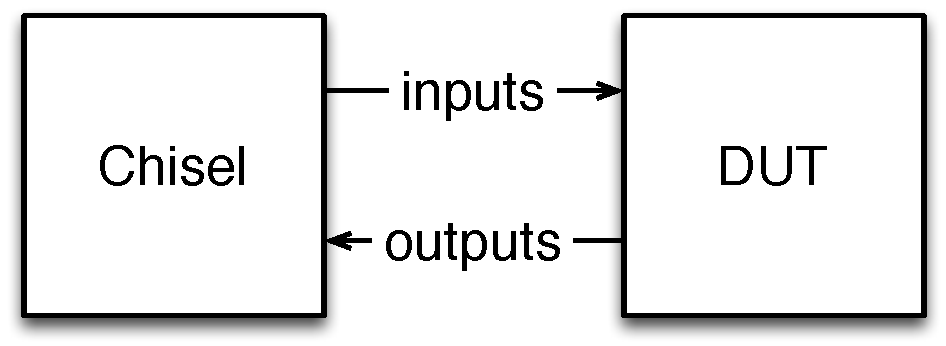
\includegraphics[width=0.45\textwidth]{../tutorial/figs/DUT.pdf}
%\end{center}
%\caption{DUT is tested under the control of Tester object}
%\label{fig:dut}
%\end{figure}

\ifbool{en}{
Testing is a crucial part of circuit design,
and thus in Chisel we provide a mechanism for
testing circuits by providing test vectors within Scala using
tester method calls
which binds a tester to a module
and allows users to write tests using the given debug protocol.  In particular, users utilize:
}
\ifbool{cn}{
测试实则是电路设计中极其关键的组成部分,因而我们在Chisel中提供可强大的测试机制,可以在Scala中提供测试向量来测试电路。
测试器被绑定到一个模块,用户可以使用如下的调试协议定义测试集,并通过调用测试器的方法来测试电路。
可以特别指出的是,用户可以使用如下测试设施:
}


\ifbool{en}{
\begin{itemize}
\item \code{poke} to set input port and state values,
\item \code{step} to execute the circuit one time unit,
\item \code{peek} to read port and state values, and
\item \code{expect} to compare peeked circuit values to expected arguments.
\end{itemize}
}
\ifbool{cn}{
\begin{itemize}
\item \code{置数操作 (poke)} :可以在输入端口和状态电路上放置数值,
\item \code{单步操作 (step)} :可以让电路往前运行一个时间单位,
\item \code{窥探操作 (peek)} :可以窥探端口和状态电路的数值,
\item \code{期待操作 (expect)} :可以用期望的参数来比较读取的电路数值。
\end{itemize}
}


\begin{commentary}
\ifbool{en}{
Chisel produces \verb$Firrtl$
intermediate representation (IR).  \verb$Firrtl$ can be interpreted directly or can be translated into \verb@Verilog@,
which can then be used to generate a C++ simulator through verilator.
}
\ifbool{cn}{
Chisel生成{\tt Firrtl}中间表示(IR),{\tt Firrtl}可以直接解释执行,也可以转换成{\tt Verilog},然后在用Verilator生成C++仿真器。
}

\end{commentary}

\ifbool{en}{
\noindent
For example, in the following:
}
\ifbool{cn}{
\noindent
例如,在下面的样本程序中,
}


\begin{scala}
class Mux2Tests(c: Mux2, b: Option[TesterBackend] = None) extends PeekPokeTester(c, _backend=b) {
  val n = pow(2, 3).toInt
  for (s <- 0 until 2) {
    for (i0 <- 0 until 2) {
      for (i1 <- 0 until 2) {
        poke(c.io.sel, s)
        poke(c.io.in1, i1)
        poke(c.io.in0, i0)
        step(1)
        expect(c.io.out, (if (s == 1) i1 else i0))
      }
    }
  }
}
\end{scala}

\ifbool{en}{
\noindent
assignments for each input of \verb+Mux2+ are set to the appropriate values using \verb+poke+. For this particular
example, we are testing the \verb+Mux2+ by hardcoding the inputs to some known values and checking
if the output corresponds to the known one. To do this, on each iteration we generate appropriate inputs
to the module and tell the simulation to assign these values to the inputs of the device we are testing \verb+c+, step
the circuit 1 clock cycle, and test the expected value. Steps are necessary to update registers and the combinational
logic driven by registers. For pure combinational paths, poke alone is sufficient to update all combinational paths
connected to the poked input wire.

Finally, the following the tester is invoked by calling \code{runPeekPokeTester}:
}
\ifbool{cn}{
\noindent
使用{\tt poke}方法,{\tt Mux2}的每个输入被赋予适当的数值。
在这个特定的例子中,我们用强硬编码的方式设置输入到某些已知的数值,然后检查输出是否是对应的已知数值,这样就可以测试{\tt Mux2}的功能。
为了实现这些测试逻辑,在每次循环中我们产生被测模块需要的恰当的输入数值,然后告诉仿真把这些数值放在我们正在测试的设备{\tt c}的输入上,向前运行电路一个时钟周期,然后用期望的结果来检查输出。
单步运行将更新寄存器和寄存器驱动的组合电路,因而是非常必要的。
对于纯组合电路路径而言,置数操作本身就足够更新所有与被置数的输入相连接的组合电路路径。

最后,通过调用函数\code{runPeekPokeTester}来激活一个测试器。
}


\begin{scala}
  def main(args: Array[String]): Unit = {
    runPeekPokeTester(() => new GCD()){
      (c,b) => new GCDTests(c,b)}
  }
\end{scala}

\ifbool{en}{
\noindent
This will run the tests defined in GCDTests with the GCD module being simulated but the \verb$Firrtl$ interpreter. We can instead have the GCD module be simulated by a C++ simulator generated by Verilator by calling the following:
}
\ifbool{cn}{
\noindent
这个例子将通过{\tt Firrtl}解释器来仿真运行\code{GCDTests}定义关于\code{GCD}的测试集。
通过下面的方法,我们也可以用Verilator生成C++仿真器来仿真\code{GCD}模块:
}


\comment{What does it mean to generate a harness file?}
\begin{scala}
  def main(args: Array[String]): Unit = {
    runPeekPokeTester(() => new GCD(), "verilator"){
      (c,b) => new GCDTests(c,b)}
  }
\end{scala}

\ifbool{en}{
\section{State Elements}
\label{sec:sequential}
}
\ifbool{cn}{
\section{状态元件}
\label{sec:sequential}
}

% SINGLE CLK and RESET

\ifbool{en}{
The simplest form of state element supported by Chisel is a
positive edge-triggered register, which can be instantiated
as:
}
\ifbool{cn}{
Chisel支持的最简单形式的状态元件就是正沿触发的寄存器,其例化方法如下:
}

\begin{scala}
val reg = Reg(next = in)
\end{scala}

\ifbool{en}{
\noindent
This circuit has an output that is a copy of the input signal \verb+in+
delayed by one clock cycle.  Note that we do not have to specify the
type of \verb+Reg+ as it will be automatically inferred from its input
when instantiated in this way.  In the current version of Chisel,
clock and reset are global signals that are implicity included where
needed.

Using registers, we can quickly define a number of useful circuit
constructs.  For example, a rising-edge detector that takes a boolean
signal in and outputs true when the current value is true and the
previous value is false is given by:
}
\ifbool{cn}{
这个电路的输出是输入信号\code{in}被延时一个时钟周期的拷贝。
请注意,我们并不需要指定\code{Reg}的数据类型,因为当用这种方式例化寄存器的时候,它的类型可以从输入那里自动推断出来。
在Chisel当前的版本,时钟和复位信号是全局信号,会被自动插入到需要的地方。

使用寄存器,我们马上就可以定义实用的电路构造了。
例如,上升沿检测器可以检测一个布尔信号的上升跳变,当输入信号的当前值为真而上一个时钟周期的值为假,检测器就会输出真。下面的电路给出了上升沿检测器的设计:
}


\begin{scala}
def risingedge(x: Bool) = x && !Reg(next = x)
\end{scala}

\ifbool{en}{
Counters are an important sequential circuit.  To construct an
up-counter that counts up to a maximum value, \verb+max+, then wraps
around back to zero (i.e., modulo \verb!max+1!), we write:
}
\ifbool{cn}{
计数器是非常重要的时序电路。
一个向上计数的计数器,在数到最大值\code{max}后会返回到零(即对\code{max+1}取模),如下方法可以实现这样的计数器:
}


\begin{scala}
def counter(max: UInt) = {
  val x = Reg(init = 0.U(max.getWidth.W))
  x := Mux(x === max, 0.U, x + 1.U)
  x
}
\end{scala}

\ifbool{en}{
\noindent
The counter register is created in the \verb!counter! function 
with a reset value of \verb!0! (with width large enough to hold \verb+max+),
to which the register will be initialized when the global reset for the circuit is asserted.
The \verb!:=! assignment to \verb!x! in \verb!counter! wires an update combinational circuit 
which increments the counter value unless it hits the \verb+max+ at which point it wraps back to zero.
Note that when \verb!x! appears on the right-hand side of
an assigment, its output is referenced, whereas when on the left-hand
side, its input is referenced.

Counters can be used to build a number of useful sequential circuits.
For example, we can build a pulse generator by outputting true when
a counter reaches zero:
}
\ifbool{cn}{
计数寄存器在函数\code{counter}中被创建出来,复位值是\code{0}(位宽恰好足够放入\code{max})。
复位值是当电路全局的复位信号有效的时候寄存器被初始化的值。
函数~\code{counter}~中的给~\code{x}~赋值的符号~\code{:=}~把一个组合电路连接到寄存器为其更新状态。
这个组合电路一直增加计数器的数值到\code{max}的时候才重新返回到零。
请注意\code{x}出现在赋值语句的右手边时,调用的是它的输出端,而当它出现在左手边时,调用的是它的输入端。

应用计数器可以构建很多有用的时序电路。
例如,我们可以构建一个脉冲发生器,在计数器返回到零的时候输出真:
}


\begin{scala}
// Produce pulse every n cycles.
def pulse(n: UInt) = counter(n - 1.U) === 0.U
\end{scala}

\ifbool{en}{
\noindent
A square-wave generator can then be toggled by the pulse train,
toggling between true and false on each pulse:
}
\ifbool{cn}{
利用在脉冲序列,反复在真和假之间反转,就可以构造方波发生器:
}


\begin{scala}[escapechar=@]
// Flip internal state when input true.
def toggle(p: Bool) = {
  val x = Reg(init = false.B)
  x := Mux(p, !x, x)
  x
}

// Square wave of a given period.
def squareWave(period: UInt) = toggle(pulse(period/2))
\end{scala}

\ifbool{en}{
\subsection{Forward Declarations}
}
\ifbool{cn}{
\subsection{前向声明}
}

\ifbool{en}{
Purely combinational circuits cannot have cycles between nodes, and
Chisel will report an error if such a cycle is detected.  Because they
do not have cycles, combinational circuits can always be constructed
in a feed-forward manner, by adding new nodes whose inputs are derived
from nodes that have already been defined.  Sequential circuits
naturally have feedback between nodes, and so it is sometimes
necessary to reference an output wire before the producing node has
been defined.  Because Scala evaluates program statements
sequentially, we allow data nodes to serve as a wire providing
a declaration of a node that can be used immediately, but whose
input will be set later.  
For example, in a simple CPU, we need to define the \verb!pcPlus4!
and \verb!brTarget! wires so they can be referenced before defined:
}
\ifbool{cn}{
纯组合电路在节点之间不能存在环,如果检测出组合逻辑环,Chisel会报错。
组合电路因为没有环,就一定可以用前馈的方式构造,新增加的节点的输入是前面定义好的节点输出。
时序电路天然地存在节点之间的反馈,因此在有的时候需要在某些节点被定义之前引用它的输出信号线。
因为Scala顺序执行程序语句,我们允许事先提供数据节点的声明,充当信号线,可以马上使用,但它的输入却在稍后给出。
例如,在下面的简单的CPU中,我们需要事先声明\code{pcPlus4}和\code{brTarget}信号线,这样它们可以在定义之前被使用。
}


\begin{scala}
val pcPlus4  = UInt()
val brTarget = UInt()
val pcNext   = Mux(io.ctrl.pcSel, brTarget, pcPlus4)
val pcReg    = Reg(next = pcNext, init = 0.U(32.W))
pcPlus4     := pcReg + 4.U
...
brTarget    := addOut
\end{scala}

\ifbool{en}{
\noindent
The wiring operator
\verb!:=! is used to wire up
the connection after \verb!pcReg! and \verb!addOut! are defined.
}
\ifbool{cn}{
在\code{pcReg}和\code{addOut}被定义之后,连线操作符~\code{:=}~连接了相关的信号。
}

\ifbool{en}{
\subsection{Conditional Updates}
}
\ifbool{cn}{
\subsection{条件更新}
}

\ifbool{en}{
In our previous examples using registers, we simply wired the
combinational logic blocks to the inputs of the registers.
When describing the operation of state
elements, it is often useful to instead specify when updates to the
registers will occur and to specify these updates spread across
several separate statements.  Chisel provides conditional update rules
in the form of the \code{when} construct to support this style of
sequential logic description. For example,
}
\ifbool{cn}{
在前面应用寄存器的例子中,我们只是简单地把组合逻辑块的输出连接到寄存器的输入。
在描述状态元件的操作时,在分立的多个语句中指出寄存器需要更新的条件是非常方便的。
Chisel提供了条件更新规则来支持这种类型的时序逻辑描述,这就是\code{when}形式的构造语法。
例如,
}
% MS: the following is not working (anymore), it results in a single bit register
% with the incrementing code.
% val r = Reg(16.U)
% MS: is there any meaning having a single, unnamed parameter for Reg()?
% MS: should this be allowed?


\begin{scala}
val r = Reg(init = 0.U(16.W))
when (cond) {
  r := r + 1.U
}
\end{scala}

\ifbool{en}{
\noindent
where register \code{r} is updated at the end of the current clock
cycle only if \verb+cond+ is \code{true}.  The argument to \code{when} is a
predicate circuit expression that returns a \code{Bool}.  The update
block following \code{when} can only contain update statements using
the assignment operator \verb+:=+, simple expressions, and named wires
defined with \code{val}.

In a sequence of conditional updates, the last conditional update
whose condition is true takes priority.  For example,
}
\ifbool{cn}{
在这个例子中寄存器\code{r}只有当\code{cond}是\code{true}的时候才在当前时钟周期结束的时候更新状态。
\code{when}语句的输入参数是一个返回\code{Bool}类型的预测电路表达式。
更新操作位于\code{when}后面的语句块中,只能包括操作符~\code{:=}~表示的赋值语句,简单的表达式和用\code{val}命名的信号线定义。

在一串条件更新语句中,最后一个条件为真的更新取得优先权。例如
}


\begin{scala}
when (c1) { r := 1.U }
when (c2) { r := 2.U }
\end{scala}

\ifbool{en}{
\noindent
leads to \code{r} being updated according to the following truth table:
}
\ifbool{cn}{
\noindent
本例中寄存器\code{r}根据下面的真值表更新状态:
}


\begin{center}
{\small
\begin{tabular}{|c|c|c|l|}
\hline
c1 & c2  &  r & \\
\hline
0 &  0 & r &  r unchanged \\
0 &  1 & 2 & \\
1 &  0 & 1 & \\
1 &  1 & 2& c2 takes precedence over c1 \\
\hline
\end{tabular}
}
\end{center}

\begin{figure}[h]
\centering
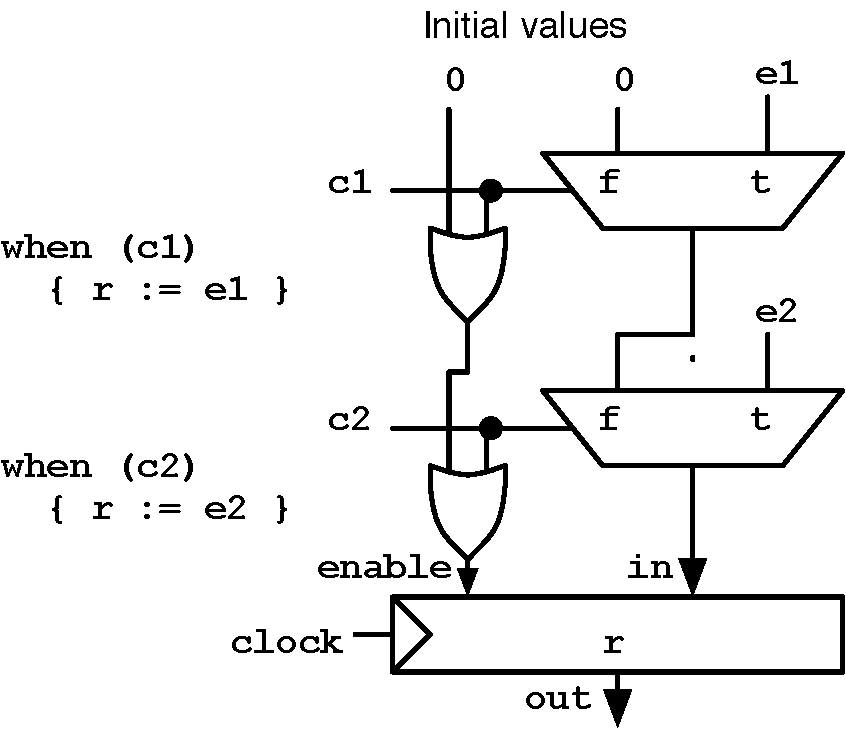
\includegraphics[width=3in]{figs/condupdates.pdf}
\ifbool{en}{
\caption{Equivalent hardware constructed for conditional updates.
  Each \code{when} statement adds another level of data mux and ORs
  the predicate into the enable chain.  The compiler effectively adds
  the termination values to the end of the chain automatically.}
}
\ifbool{cn}{
\caption{本例中一串条件更新语句构造的等价电路。每一个\code{when}语句增加新的一级数据多路选择器,它们的条件用逻辑或门串在一起组成寄存器的使能信号。Chisel编译器会在逻辑或门链的结尾自动加入终止数值。}
}


\label{fig:condupdates}
\end{figure}

\ifbool{en}{
Figure~\ref{fig:condupdates} shows how each conditional update can be
viewed as inserting a mux before the input of a register to select
either the update expression or the previous input according to the
\code{when} predicate.  In addition, the predicate is OR-ed into an
enable signal that drives the load enable of the register.  The
compiler places initialization values at the beginning of the chain so
that if no conditional updates fire in a clock cycle, the load enable
of the register will be deasserted and the register value will not
change.
}
\ifbool{cn}{
图\ref{fig:condupdates} 表明每一个条件更新语句都可以被看作是在寄存器的输入前面插入了一个多路选择器,根据\code{when}语句的条件,或者选择更新表达式或者选择上一个输入。
而且这些条件或在一起成为使能信号接入到寄存器的加载使能信号上。
编译器在逻辑或门链的开始放置初始值,这样如果在本时钟周期内没有条件更新被激活,寄存器的加载使能端就被置为无效,寄存器的值也就不会发生改变。
}


\ifbool{en}{
Chisel provides some syntactic sugar for other common forms of
conditional update.  The \verb+unless+ construct is the same as
\verb+when+ but negates its condition.  In other words,
}
\ifbool{cn}{
Chisel为条件更新的一些普遍的形式提供了一些语法糖。
\code{unless}语句与\code{when}语句类似,但是在它们生效的条件相反。
换言之,
}


\begin{scala}
unless (c) { body }
\end{scala}
\ifbool{en}{
is the same as
}
\ifbool{cn}{
等效于
}


\begin{scala}
when (!c) { body }
\end{scala}

% The \verb+otherwise+ construct is the same as \verb+when+ with a true
% condition.  In other words,
% \begin{scala}
% otherwise { body }
% \end{scala}
% 
% \noindent
% is the same as
% \begin{scala}
% when (true.B) { body }
% \end{scala}

\ifbool{en}{
The update block can target multiple registers, and there can be
different overlapping subsets of registers present in different update
blocks.  Each register is only affected by conditions in which it
appears.  The same is possible for combinational circuits (update
of a \code{Wire}). Note that all combinational
circuits need a default value. For example:
}
\ifbool{cn}{
更新语句块可以操作多个寄存器,而且这组寄存器多个不同的相互重叠的子集可以出现在多个更新语句块中。
只有包裹了寄存器更新语句块的条件才会影响这个寄存器的后续值。
同样的原则也适用于组合逻辑电路中(更新一个\code{Wire}类型的信号线)。
需要注意的是,所有组合电路的信号线需要一个默认的值。
例如,
}


\begin{scala}
r := 3.S; s := 3.S
when (c1)   { r := 1.S; s := 1.S }
when (c2)   { r := 2.S }
\end{scala}

\ifbool{en}{
\noindent
leads to \code{r} and \code{s} being updated according to the
following truth table:
}\ifbool{cn}{
\noindent
这段代码中\code{r}和\code{s}根据如下的真值表更新状态:
}



\begin{scala}
c1 c2  r  s
0   0  3  3
0   1  2  3 // r updated in c2 block, s at top level.
1   0  1  1
1   1  2  1
\end{scala}


\begin{commentary}
\ifbool{en}{
We are considering adding a different form of conditional update,
where only a single update block will take effect.  These atomic
updates are similar to Bluespec guarded atomic actions.
}\ifbool{cn}{
我们也在考虑增加另一种条件更新的形式,只允许单个更新块发生作用。
这些原子更新操作将会非常像Bluespec中的受保护的原子操作。
}


%TODO: when / .elsewhen / .otherwise
\end{commentary}

\ifbool{en}{
Conditional update constructs can be nested and any given block is
executed under the conjunction of all outer nesting conditions.  For
example,
}\ifbool{cn}{
条件更新构造表达式块可以嵌套,某一表达式块在其所有嵌套在外边的条件都满足的时候才会被执行。
例如
}


\begin{scala}
when (a) { when (b) { body } }
\end{scala}

\ifbool{en}{
\noindent
is the same as:
}\ifbool{cn}{
\noindent
等效于
}


\begin{scala}
when (a && b) { body }
\end{scala}

\ifbool{en}{
Conditionals can be chained together using
\verb+when+, \verb+.elsewhen+, \verb+.otherwise+ corresponding to
\verb+if+, \verb+else if+ and \verb+else+ in Scala.  For example,
}\ifbool{cn}{
多个条件可以用
\code{when}, \code{.elsewhen}, \code{.otherwise}
串在一起,就像Scala语言中的
\code{if}, \code{else if} 和 \code{else}。
}


\begin{scala}
when (c1) { u1 }
.elsewhen (c2) { u2 }
.otherwise { ud }
\end{scala}
\ifbool{en}{
\noindent
is the same as:
}\ifbool{cn}{
\noindent
等效于
}


\begin{scala}
when (c1) { u1 }
when (!c1 && c2) { u2 }
when (!(c1 || c2)) { ud }
\end{scala}

\ifbool{en}{
We introduce the \code{switch} statement for conditional updates
involving a series of comparisons against a common key.  For example,
}\ifbool{cn}{
当处理针对一个共同的键值一系列比较的时候,我们还为条件更新引入了\code{switch}语法。
例如,
}


\begin{scala}
switch(idx) {
 is(v1) { u1 }
 is(v2) { u2 }
}
\end{scala}
\ifbool{en}{
\noindent
is equivalent to:
}\ifbool{cn}{
等效于:
}


\begin{scala}
when (idx === v1) { u1 }
.elsewhen (idx === v2) { u2 }
\end{scala}


\ifbool{en}{
Chisel also allows a \code{Wire}, i.e., the output of some
combinational logic, to be the target of conditional update statements
to allow complex combinational logic expressions to be built
incrementally.  Chisel does not allow a combinational output to be
incompletely specified and will report an error if an unconditional
update is not encountered for a combinational output.
}\ifbool{cn}{
\code{Wire}类型表示的是组合逻辑电路的输出信号线,Chisel也允许条件更新语句式用于\code{Wire}类型的数据,这样复杂的组合逻辑表达式就可以递增地构建出来。
Chisel要求组合电路输出的更新条件必须是完全的,如果组合电路输出没有默认的更新规则,Chisel会报错。
}


\begin{commentary}
\ifbool{en}{
In Verilog, if a procedural specification of a combinational logic
block is incomplete, a latch will silently be inferred causing many
frustrating bugs.
}\ifbool{cn}{
在Verilog中,如果组合逻辑块的程序性的规范是不完全的,一个锁存器就被静悄悄的产生了,这导致了大量的令人抓狂的缺陷。
}


\ifbool{en}{
It could be possible to add more analysis to the Chisel compiler, to
determine if a set of predicates covers all possibilities.  But for
now, we require a single predicate that is always true in the
chain of conditional updates to a \code{Wire}.
}\ifbool{cn}{
为了确定一组更新条件是否覆盖了所有的可能性,在Chisel的编译器内加入更多的分析本是可行的。
但是现在的版本中,我们需要在\code{Wire}类型的条件更新链条的一开始加入一个条件为真的默认更新规则。
}


\end{commentary}

\ifbool{en}{
\subsection{Finite State Machines}
}\ifbool{cn}{
\subsection{有限状态机}
}

\ifbool{en}{
A common type of sequential circuit used in digital design is a Finite
State Machine (FSM).  An example of a simple FSM is a parity
generator:
}\ifbool{cn}{
在数字电路设计中,一种常见的时序电路类型就是状态机(FSM)。
奇偶发生器就是FSM的一个简单例子:
}

% \begin{scala}
% class Parity extends Module {
%   val io = IO(new Bundle {
%     val in  = Input(Bool())
%     val out = Output(Bool()) })
%   val s_even :: s_odd :: Nil = Enum(2)
%   val state  = Reg(init = s_even)
%   switch(state, Array(
%     (s_even, () => { when (io.in) { state := s_odd } }),
%     (s_odd,  () => { when (io.in) { state := s_even } }) ))
%   io.out := state === s_odd
% }
% \end{scala}

\begin{scala}
class Parity extends Module {
  val io = IO(new Bundle {
    val in  = Input(Bool())
    val out = Output(Bool()) })
  val s_even :: s_odd :: Nil = Enum(2)
  val state  = Reg(init = s_even)
  when (io.in) {
    when (state === s_even) { state := s_odd  }
    when (state === s_odd)  { state := s_even }
  }
  io.out := (state === s_odd)
}
\end{scala}

\ifbool{en}{
\noindent
where \verb+Enum(2)+ generates two \verb+UInt+ literals.
States are updated when \verb+in+ is true.  It is worth
noting that all of the mechanisms for FSMs are built upon registers,
wires, and conditional updates.
}\ifbool{cn}{
\noindent
这里\code{Enum(2)}生成两个\code{UInt}类型的字面常量。
当输入信号\code{in}为真的时候,状态才会被更新。
值得特别提及的是,FSM所有的构造机制都建立在寄存器、信号线和条件更新之上。
}


\ifbool{en}{
Below is a more complicated FSM example which is a circuit for
accepting money for a vending machine:
}\ifbool{cn}{
下面给出了一个稍微复杂点儿的FSM例子,这是为自动售货机如何收钱而设计的一个电路:
}


\begin{scala}
class VendingMachine extends Module {
  val io = IO(new Bundle {
    val nickel = Input(Bool())
    val dime   = Input(Bool())
    val valid    = Output(Bool()) })
  val s_idle :: s_5 :: s_10 :: s_15 :: s_ok :: Nil = Enum(5)
  val state = Reg(init = s_idle)
  when (state === s_idle) {
    when (io.nickel) { state := s_5 }
    when (io.dime)   { state := s_10 }
  }
  when (state === s_5) {
    when (io.nickel) { state := s_10 }
    when (io.dime)   { state := s_15 }
  }
  when (state === s_10) {
    when (io.nickel) { state := s_15 }
    when (io.dime)   { state := s_ok }
  }
  when (state === s_15) {
    when (io.nickel) { state := s_ok }
    when (io.dime)   { state := s_ok }
  }
  when (state === s_ok) {
    state := s_idle
  }
  io.valid := (state === s_ok)
}
\end{scala}

\ifbool{en}{
\noindent
Here is the vending machine FSM defined with \code{switch} statement:
}\ifbool{cn}{
下面再给出用\code{switch}语句设计的自动售货机的FSM:
}


\begin{scala}
class VendingMachine extends Module {
  val io = IO(new Bundle {
    val nickel = Input(Bool())
    val dime   = Input(Bool())
    val valid  = Output(Bool())
  })
  val s_idle :: s_5 :: s_10 :: s_15 :: s_ok :: Nil = Enum(5)
  val state = Reg(init = s_idle)
  
  switch (state) {
    is (s_idle) {
      when (io.nickel) { state := s_5 }
      when (io.dime) { state := s_10 }
    }
    is (s_5) {
      when (io.nickel) { state := s_10 }
      when (io.dime) { state := s_15 }
    }
    is (s_10) {
      when (io.nickel) { state := s_15 }
      when (io.dime) { state := s_ok }
    }
    is (s_15) {
      when (io.nickel) { state := s_ok }
      when (io.dime) { state := s_ok }
    }
    is (s_ok) {
      state := s_idle
    }
  }
  io.valid := (state === s_ok)
}
\end{scala}


\ifbool{en}{
\section{Memories}
}\ifbool{cn}{
\section{存储器}
}


\ifbool{en}{
Chisel provides facilities for creating both read only and
read/write memories.  
}\ifbool{cn}{
Chisel提供了创建只读存储器和可读写存储器的机制。
}

\ifbool{en}{
\subsection{ROM}
}\ifbool{cn}{
\subsection{只读存储器(ROM)}
}

\ifbool{en}{
Users can define read only memories with a \code{Vec}:
}\ifbool{cn}{
用户可以使用\code{Vec}类型来定义只读存储器,如示例:
}


\begin{scala}
Vec(inits: Seq[T])
Vec(elt0: T, elts: T*)
\end{scala}

\ifbool{en}{
\noindent
where \verb+inits+ is a sequence of initial \verb+Data+ literals that
initialize the ROM.
For example,  users can
create a small ROM initialized to \verb+1, 2, 4, 8+ and 
loop through all values using a counter as an address generator as follows:
}\ifbool{cn}{
\noindent
这里\code{inits}是一串初始\code{Data}类型的字面常量,用来初始化ROM。
用户可以创建一个小ROM,初始化成\code{1, 2, 4, 8},并且用一个计数器作为地址生成器来遍历它所有的值,如下例所示:
}


\begin{scala}
val m = Vec(Array(1.U, 2.U, 4.U, 8.U))
val r = m(counter(UInt(m.length.W)))
\end{scala}

\ifbool{en}{
\noindent
We can create an \verb+n+ value sine lookup table using a ROM initialized as follows:
}\ifbool{cn}{
\noindent
我们可以ROM创建一个有\code{n}个入口的sine函数的查找表,如下例所示:
}


\begin{scala}
def sinTable (amp: Double, n: Int) = {
  val times = 
    Range(0, n, 1).map(i => (i*2*Pi)/(n.toDouble-1) - Pi)
  val inits = 
    times.map(t => SInt(round(amp * sin(t)), width = 32))
  Vec(inits)
}
def sinWave (amp: Double, n: Int) = 
  sinTable(amp, n)(counter(UInt(n.W))
\end{scala}

\ifbool{en}{
\noindent
where \verb+amp+ is used to scale the fixpoint values stored in the ROM.
}\ifbool{cn}{
\noindent
这里的\code{amp}用来缩放ROM中保存的定点数值。
}


\ifbool{en}{
\subsection{Mem}
}\ifbool{cn}{
\subsection{可读写存储器(Mem)}
}


\ifbool{en}{
Memories are given special treatment in Chisel since hardware
implementations of memory have many variations, e.g., FPGA memories
are instantiated quite differently from ASIC memories.  Chisel defines
a memory abstraction that can map to either simple Verilog behavioral
descriptions, or to instances of memory modules that are available
from external memory generators provided by foundry or IP vendors.  

Chisel supports random-access memories via the \code{Mem} construct.
Writes to Mems are positive-edge-triggered and reads are either
combinational or positive-edge-triggered.\footnote{Current FPGA technology
does not support combinational (asynchronous) reads (anymore). The read address
needs to be registered.}


Ports into Mems are created by applying a \code{UInt} index.  A 32-entry
register file with one write port and two combinational read ports might be
expressed as follows:
}\ifbool{cn}{
可读写存储器有很多种硬件实现方法,比如,FPGA的存储器就和ASIC的实例化方法就非常不同,因而Chisel给予存储器很特别的待遇。
Chisel定义了一种抽象的存储器,既可以映射到简单的Verilog行为描述,也可以映射到代工厂或IP供货商给出的存储器模块的实例。

Chisel通过\code{Mem}构造器来支持随机访问的存储器。
写入存储器是正沿触发的行为,读取存储器可以是组合逻辑输出,也可以是正沿触发的行为。
\footnote{现在的FPGA工艺已经不(再)支持组合逻辑(异步)读取存储器了。读地址需要用寄存器锁住。}
}


\begin{scala}
val rf = Mem(32, UInt(64.W))
when (wen) { rf(waddr) := wdata }
val dout1 = rf(waddr1)
val dout2 = rf(waddr2)
\end{scala}

\ifbool{en}{
If the optional parameter \code{seqRead} is set, Chisel will attempt to infer
sequential read ports when the read address is a \code{Reg}.  A one-read port,
one-write port SRAM might be described as follows:
}\ifbool{cn}{
在可选参数\code{seqRead}被设置成有效的时候,如果读地址是一个\code{Reg},Chisel就会尝试推断时序读端口。
单个读端口、单个写端口的SRAM可以如下设计:
}


\begin{scala}
val ram1r1w =
  Mem(1024, UInt(32.W))
val reg_raddr = Reg(UInt())
when (wen) { ram1r1w(waddr) := wdata }
when (ren) { reg_raddr := raddr }
val rdata = ram1r1w(reg_raddr)
\end{scala}

\ifbool{en}{
Single-ported SRAMs can be inferred when the read and write conditions are
mutually exclusive in the same \code{when} chain:
}\ifbool{cn}{
如果读取和写入被放在在同一个\code{when}语句中,并且它们的条件是互斥的,那么就可以推断这是一个单端口SRAM。
}


\begin{scala}
val ram1p = Mem(1024, UInt(32.W))
val reg_raddr = Reg(UInt())
when (wen) { ram1p(waddr) := wdata }
.elsewhen (ren) { reg_raddr := raddr }
val rdata = ram1p(reg_raddr)
\end{scala}

\ifbool{en}{
If the same \code{Mem} address is both written and sequentially read on the same clock
edge, or if a sequential read enable is cleared, then the read data is
undefined.

\code{Mem} also supports write masks for subword writes.  A given bit is written if
the corresponding mask bit is set.
}\ifbool{cn}{
如果在同一个时钟周期,同时写入和读取相同的\code{Mem}地址,那么读出的数据是未定义的。
如果时序读取的使能是无效的,那么读出的数据也是未定义的。

\code{Mem}也支持写入模具来实现部分写入操作。
只有当对应的写入模具的比特有效的时候,给定的比特才会被写入存储器。
}


\begin{scala}
val ram = Mem(256, UInt(32.W))
when (wen) { ram.write(waddr, wdata, wmask) }
\end{scala}


% For example, an
% audio recorder could be defined as follows:
% 
% \begin{scala}
%   def audioRecorder(n: Int, button: Bool) = { 
%     val addr   = counter(UInt(n.W))
%     val ram    = Mem(n)
%     ram(addr) := button
%     ram(Mux(button(), 0.U, addr))
%   } 
% \end{scala}
% 
% \noindent
% where a counter is used as an address generator into a memory.  
% The device records while \verb+button+ is \verb+true+, or plays back when \verb+false+.


\ifbool{en}{
\section{Interfaces \& Bulk Connections}
\label{sec:interfaces}
}\ifbool{cn}{
\section{接口和成批连接}
}


\ifbool{en}{
For more sophisticated modules it is often useful to define and
instantiate interface classes while defining the IO for a module.  First and
foremost, interface classes promote reuse allowing users to capture
once and for all common interfaces in a useful form.  Secondly,
interfaces allow users to dramatically reduce wiring by supporting
{\em bulk connections} between producer and consumer modules.  Finally,
users can make changes in large interfaces in one place reducing the
number of updates required when adding or removing pieces of the
interface.
}\ifbool{cn}{
对于复杂的电路模块来说,定义和例化接口类是非常有效的设计模块IO的方法。
首先最重要的,接口类允许用户用有效的形式化的方法抓住那些能够设计一次复用多次的接口,鼓励他们复用设计。
再者,接口支持在生产者和消费者模块之间使用{\em 成批连接},允许用户大幅节省连线语句。
最后,用户可以在管理大接口变动的时候只在一处做更改,在增加减少接口子域的时候减少了更改的位置数量。
}

\ifbool{en}{
\subsection{Ports: Subclasses  \& Nesting}
}\ifbool{cn}{
\subsection{端口:子类和嵌套}
}

\ifbool{en}{
As we saw earlier, users can define their own interfaces by defining a class that subclasses \verb+Bundle+.  
For example, a user could define a simple link for handshaking data as follows:
}\ifbool{cn}{
如我们之前讨论过的,用户可以从\code{Bundle}继承子类来定义自己的接口。
例如,用户可以像这样定一个简单的链路来传输握手数据:
}


\begin{scala}
class SimpleLink extends Bundle { 
  val data  = Output(UInt(16.W)) 
  val valid = Output(Bool())
}
\end{scala}

\ifbool{en}{
\noindent
We can then extend \verb+SimpleLink+ by adding parity bits using
bundle inheritance:
}\ifbool{cn}{
\noindent
我们下面可以用继承的方法增加奇偶位来扩展\code{SimpleLink}:
}


\begin{scala}
class PLink extends SimpleLink { 
  val parity = Output(UInt(5.W)) 
}
\end{scala}

\ifbool{en}{
\noindent
In general, users can organize their interfaces into hierarchies using inheritance.  

From there we can define a filter interface by nesting two
\verb+PLink+s into a new \verb+FilterIO+ bundle:
}\ifbool{cn}{
\noindent
一般来说,用户可以用继承的方法组织出层级化的接口。

现在,只要把两个\code{PLink}套叠在一起形成新的绑裹\code{FilterIO},我们就可以定义过滤器接口了:
}


\begin{scala}
class FilterIO extends Bundle { 
  val x = new PLink().flip
  val y = new PLink()
}
\end{scala}

\ifbool{en}{
\noindent
where \verb+flip+ recursively changes the ``gender'' of a bundle,
changing input to output and output to input.

We can now define a filter by defining a filter class extending module:
}\ifbool{cn}{
\noindent
这里\code{flip}逐级递归地反转一个绑裹内部成员的“性别”,把输入变成输出,输出变成输入。

现在我们可以从模块继承一个过滤器类来定义过滤器了:
}


\begin{scala}
class Filter extends Module { 
  val io = IO(new FilterIO())
  ...
}
\end{scala}

\ifbool{en}{
\noindent 
where the \verb+io+ field contains \verb+FilterIO+. 
}\ifbool{cn}{
\noindent
这里\code{FilterIO}构成了模块的\code{io}域。
}


\ifbool{en}{
\subsection{Bundle Vectors}
}\ifbool{cn}{
\subsection{向量绑裹}
}


\ifbool{en}{
Beyond single elements, vectors of elements form richer hierarchical interfaces.  
For example, in order to create a crossbar with a vector of inputs, producing a vector of outputs, and selected by a UInt input, 
we utilize the \verb+Vec+ constructor:
}\ifbool{cn}{
元素的向量超过单个元素,可以形成更加丰富的接口层级。
例如,根据一个\code{UInt}输入从一组输入生成一组输入的交换器可以通过\code{Vec}构造器实现:
}


\begin{scala}
class CrossbarIo(n: Int) extends Bundle {
  val in  = Vec(n, new PLink().flip())
  val sel = Input(UInt(sizeof(n).W))
  val out = Vec(n, new PLink())
}
\end{scala}

% \begin{scala}
% class CrossbarIo(n: Int) extends Bundle {
%   val in  = Vec(n, Input(UInt(w.W)))
%   val sel = Vec(n, Input(UInt(sizeof(n).W)))
%   val out = Vec(n, Output(UInt(w.W)))
% }
% \end{scala}

\ifbool{en}{
\noindent
where \verb+Vec+ takes a size as the first argument and a block returning a port as the second argument.
}\ifbool{cn}{
\noindent
这里\code{Vec}的第一个参数规定了数量,第二个参数是能产生端口的语句块。
}


\ifbool{en}{
\subsection{Bulk Connections}
}\ifbool{cn}{
\subsection{成批连接}
}

\ifbool{en}{
We can now compose two filters into a filter block as follows:
}\ifbool{cn}{
现在我们来用两个过滤来组成一个过滤器丛,如下例所示:
}

\begin{scala}
class Block extends Module { 
  val io = IO(new FilterIO())
  val f1 = Module(new Filter())
  val f2 = Module(new Filter())

  f1.io.x <> io.x
  f1.io.y <> f2.io.x
  f2.io.y <> io.y
}
\end{scala}

\ifbool{en}{
\noindent
where \verb+<>+ bulk connects interfaces of opposite gender between
sibling modules or interfaces of same gender between parent/child modules. 
Bulk connections connect leaf ports of the same name to each other.
After all connections are made and the circuit is being elaborated,
Chisel warns users if ports have other than exactly one connection to them.
}\ifbool{cn}{
\noindent  
这里\code{<>}就是成批连接的操作符,它可以把两个子模块的相对方向的端口连接起来,也可以把父模块和子模块的相同方向的端口连接起来。
成批连接能够把相同名字的子端口相互连接起来。
当所有的连接都成功之后,电路就开始详细展开了。
如果有端口被连接了多个端口,Chisel就会报告警告给用户。
}


\ifbool{en}{
\subsection{Interface Views}
}\ifbool{cn}{
\subsection{接口的视域}
}


\begin{figure}
\centerline{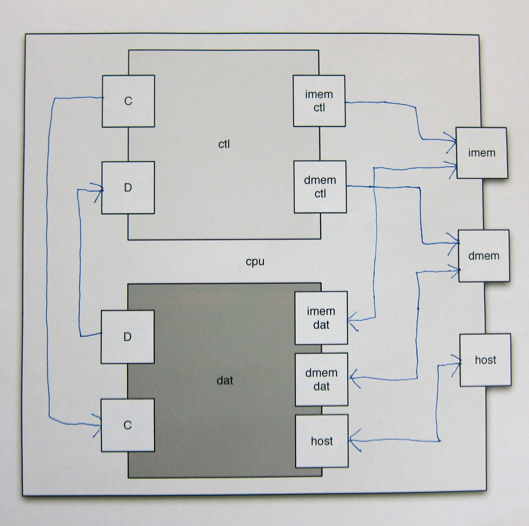
\includegraphics[width=3in]{figs/cpu.png}}
\ifbool{en}{
\caption{Simple CPU involving control and data path submodules and host and memory interfaces.}
}\ifbool{cn}{
\caption{包含控制、数据子模块和和主控、存储器接口的简化的CPU。}
}

\label{fig:cpu}
\end{figure}

\ifbool{en}{
Consider a simple CPU consisting of control path and data path submodules and host and memory interfaces shown in Figure~\ref{fig:cpu}.
In this CPU we can see that the control path and data path each connect only to a part of the instruction and data memory interfaces. 
Chisel allows users to do this with partial fulfillment of interfaces.
A user first defines the complete interface to a ROM and Mem as follows:
}\ifbool{cn}{
如图~\ref{fig:cpu} 所示,考虑一个简化的CPU,只包括控制、数据子模块和和主控、存储器接口。
在这个CPU中我们看到,控制通路和数据通路都只和指令和数据存储器接口的一部分连在一起。
Chisel允许用户局部地填充接口。
用户先这样定义只读存储器和可读写存储器的完整的接口:
}


\begin{scala}
class RomIo extends Bundle {
  val isVal = Input(Bool())
  val raddr = Input(UInt(32.W))
  val rdata = Output(UInt(32.W))
}

class RamIo extends RomIo {
  val isWr  = Input(Bool())
  val wdata = Input(UInt(32.W))
}
\end{scala}

\ifbool{en}{
\noindent
Now the control path can build an interface in terms of these interfaces:
}\ifbool{cn}{
\noindent
现在控制通路可以用这些接口来定义自己的接口。
}


\begin{scala}
class CpathIo extends Bundle {
  val imem = RomIo().flip()
  val dmem = RamIo().flip()
  ...
}
\end{scala}

\ifbool{en}{
\noindent
and the control and data path modules can be built by partially assigning to
this interfaces as follows:
}\ifbool{cn}{
\noindent
控制通路和数据通路模块可以部分地连接这些端口,如示:
}


\begin{scala}
class Cpath extends Module {
  val io = IO(new CpathIo())
  ...
  io.imem.isVal := ...
  io.dmem.isVal := ...
  io.dmem.isWr  := ...
  ...
}

class Dpath extends Module {
  val io = IO(new DpathIo())
  ...
  io.imem.raddr := ...
  io.dmem.raddr := ...
  io.dmem.wdata := ...
  ...
}
\end{scala}

\ifbool{en}{
\noindent
We can now wire up the CPU using bulk connects as we would with other bundles:
}\ifbool{cn}{
\noindent
现在我们可以在CPU模块中按照我们设想的那样使用成批连接了:
}


\begin{scala}
class Cpu extends Module {
  val io = IO(new CpuIo())
  val c  = Module(new CtlPath())
  val d  = Module(new DatPath())
  c.io.ctl  <> d.io.ctl
  c.io.dat  <> d.io.dat
  c.io.imem <> io.imem
  d.io.imem <> io.imem
  c.io.dmem <> io.dmem
  d.io.dmem <> io.dmem
  d.io.host <> io.host
}
\end{scala}

\ifbool{en}{
\noindent
Repeated bulk connections of partially assigned control and data path interfaces
completely connect up the CPU interface.
}\ifbool{cn}{
\noindent
重复的成批连接分别在局部连接了控制通路和数据通路的接口,最终把CPU的接口完全的连接起来。
}

% A Bool can be automatically treated as a single bit UInt (with values
% 0 or 1), but an Int or UInt cannot be used as a Bool without an
% explicit cast.
%
%   Lit(5) // means a constant node with decimal value 5. Bit width will
%           // be inferred automatically if possible
%
% A node is a hardware operator that has zero or more inputs and that
% drives one output.  An example of a node with zero inputs is a
% constant generator.
%
% \begin{scala}
% Lit(10, 4) // means a constant node of type UInt that is 4 bits
%            // wide with decimal 10.
% Lit(10)
% LitInt(10, 4)
% LitUInt(10, 4)
% Lit(-1,4)
% \end{scala}
%
% can more concisely write:
%
% Module correspond to Verilog modules
% Cell is a sub-module, Chisel Module


\ifbool{en}{
\section{Functional Module Creation}
\label{sec:funconstructor}
}\ifbool{cn}{
\section{函数式的模块创建}
\label{sec:funconstructor}
}

\ifbool{en}{
It is also useful to be able to make a functional interface for
module construction.  For instance, we could build a constructor
that takes multiplexer inputs as parameters and returns the
multiplexer output:
}\ifbool{cn}{
为模块构造设计一个函数式的接口也是非常有用的。
例如,我们可以设计一个构造器,它以多路选择器模块作为输入,以更复杂的多路选择器模块作为输出:
}


\begin{scala}
object Mux2 {
  def apply (sel: UInt, in0: UInt, in1: UInt) = {
    val m = new Mux2()
    m.io.in0 := in0
    m.io.in1 := in1
    m.io.sel := sel
    m.io.out
  }
}
\end{scala}

\ifbool{en}{
\noindent
where \code{object Mux2} creates a Scala singleton object on the \code{Mux2}
module class, and \code{apply} defines a method for creation of a \code{Mux2} instance.
%
With this \code{Mux2} creation function, the specification of \code{Mux4} now is
significantly simpler.
}\ifbool{cn}{
\noindent
这里\code{object Mux2}是在模块类\code{Mux2}的基础上创建的一个Scala单例对象,\code{apply}定义了一个方法可以创建一个\code{Mux2}的实例。
有了这个\code{Mux2}创建函数,\code{Mux4}的设计规范就显著的简单了。
}


\begin{scala}
class Mux4 extends Module {
  val io = IO(new Bundle {
    val in0 = Input(UInt(1.W))
    val in1 = Input(UInt(1.W))
    val in2 = Input(UInt(1.W))
    val in3 = Input(UInt(1.W))
    val sel = Input(UInt(2.W))
    val out = Output(UInt(1.W))
  })
  io.out := Mux2(io.sel(1),
                 Mux2(io.sel(0), io.in0, io.in1),
                 Mux2(io.sel(0), io.in2, io.in3))
}
\end{scala}

\ifbool{en}{
Selecting inputs is so useful that Chisel builds it in and calls it
\code{Mux}.  However, unlike \code{Mux2} defined above, the builtin version allows any datatype on
\code{in0} and \code{in1} as long as they are the same subclass of \code{Data}.
In Section~\ref{sec:parameterization} we will see how to define this
ourselves.

Chisel provides \code{MuxCase} which is an n-way \code{Mux} 
}\ifbool{cn}{
从输入中做多路选择是如此的重要,所以Chisel把这个功能内建了,这就是\code{Mux}。
然而,不同于上面设计的\code{Mux2},Chisel内建的版本允许\code{in0}和\code{in1}是任何数据类型,只要它们都属于继承于\code{Data}的相同子类。
在第~\ref{sec:parameterization}~节,我们会看到如何自己定义这样的高阶版本。
}


\begin{scala}
MuxCase(default, Array(c1 -> a, c2 -> b, ...))
\end{scala}
 
\ifbool{en}{
\noindent
where each condition / value is represented as a tuple in a Scala
array and where \code{MuxCase} can be translated into the following
\code{Mux} expression:
}\ifbool{cn}{
\noindent
此处的每个条件~/~数值的被表示成Scala数组中的三元组,\code{MuxCase}可以被翻译成下面的\code{Mux}表达式。
}

\begin{scala}
Mux(c1, a, Mux(c2, b, Mux(..., default)))
\end{scala}

\ifbool{en}{
\noindent
Chisel also provides \code{MuxLookup} which is an n-way indexed multiplexer:
}\ifbool{cn}{
\noindent
Chisel还提供了\code{MuxLookup},这是一个n路的多路选择器:
}

\begin{scala}
MuxLookup(idx, default, 
          Array(0.U -> a, 1.U -> b, ...))
\end{scala}

\ifbool{en}{
\noindent
which can be rewritten in terms of:\verb+MuxCase+ as follows:
}\ifbool{cn}{
\noindent
它可以用\code{MuxCase}重新写成下面的形式:
}

\begin{scala}
MuxCase(default, 
        Array((idx === 0.U) -> a,
              (idx === 1.U) -> b, ...))
\end{scala}

\ifbool{en}{
\noindent
Note that the cases (eg. c1, c2) must be in parentheses.
}\ifbool{cn}{
\noindent
请注意,这些条件(如c1, c2)必须用小括号括起来。
}

% TODO: higher order filter

% \Noindent
% where the overall expression returns the value corresponding to the first condition evaluating to true.

% FUNCTIONAL CREATION
%
% want to go from io to constructor
%
% \begin{scala}
% val io = IO(new Bundle{
%   val sel = Input(UInt(1.W))
%   val in0 = Input(UInt(1.W))
%   val in1 = Input(UInt(1.W))
%   val out = Output(UInt(1.W))
% })
% def Mux2(sel: UInt, in0: UInt, in0: UInt): UInt = {
%   val m = new Mux2()
%   m.io.wire(Array("sel" => sel, "in0" => in0, "in1" => in1), "out")
% }
% \end{scala}

% picture of box in box

%%%%%%%%%%%%%%%%%%%%%%%%%%%%%%%%%%%%%%%%%%%%%%%%%%%%%%%%%%%%%%%%%%%%%%%%%%%%%%%%%%%%%%%%%%%%%%%%%%%%%%%%%%%%%%
\ifbool{en}{
\section{Polymorphism and \newline Parameterization}
\label{sec:parameterization}
}\ifbool{cn}{
\section{多态和参数化设计}
\label{sec:parameterization}
}

\ifbool{en}{
Scala is a strongly typed language and uses parameterized types to specify generic functions and classes.  
In this section, we show how Chisel users can define their own reusable functions and classes using parameterized classes.
}\ifbool{cn}{
Scala是强类型的语言,可以用参数化的数据类型来定义一般化的函数和类。
在本节,我们会展示Chisel的用户如何能够用参数化的类来设计他们自己的可复用的函数和类。
}


\begin{commentary}
\ifbool{en}{
This section is advanced and can be skipped at first reading.
}\ifbool{cn}{
本节是教程的高阶部分,初次阅读可以跳过。
}


\end{commentary}

\ifbool{en}{
\subsection{Parameterized Functions}
}\ifbool{cn}{
\subsection{参数化的函数}
}

\ifbool{en}{
Earlier we defined \code{Mux2} on \code{Bool}, but now we show how we can define a generic multiplexer function.
We define this function as taking a boolean condition and con and alt arguments (corresponding to then and else expressions) of type \code{T}:
}\ifbool{cn}{
前面我们使用\code{Bool}类型定义了\code{Mux2},现在我们来看一下如何定一个一般化的多路选择器函数。
我们以布尔类型的条件和\code{T}类型的数据con和alt为参数来定义这个一般化的函数(con和alt分别表示then和else表达式)。
}


\begin{scala}
def Mux[T <: Bits](c: Bool, con: T, alt: T): T { ... }
\end{scala}

\ifbool{en}{
\noindent
where \code{T} is required to be a subclass of \code{Bits}.
Scala ensures that in each usage of \code{Mux}, it can find a common superclass of the actual con and alt argument types, 
otherwise it causes a Scala compilation type error.
For example,
}\ifbool{cn}{
\noindent
这里的\code{T}必须是\code{Bits}类型的子类。
Scala在调用\code{Mux}的时候会确保它能够找到实际的con和alt的参数类型共同的超类,否则它会报告编译时期的类型错误。
例如,
}


\begin{scala}
Mux(c, 10.U, 11.U)
\end{scala}

\ifbool{en}{
\noindent
yields a \code{UInt} wire because the \code{con} and \code{alt} arguments are each of type \code{UInt}.
}\ifbool{cn}{
将生成一个\code{UInt}类型的信号线,这是因为此处的\code{con}和\code{alt}参数都属于\code{UInt}类型。
}

% Earlier we defined \code{Mux2} on \code{Bool}, but now we show how we can define a generic \code{Mux}.  
% We define a function that takes a condition and two functions of no arguments (called thunks) for the {\it then} and {\it else} cases:
% 
% \begin{scala}
% def Mux[T <: UInt](c: Bool, con: T, alt: T): T
% def Mux[T <: UInt](c: Bool)(con: => T)(alt: => T): T
% \end{scala}
% 
% \noindent
% where the two thunk return types are parameterized to be a type \code{T} that is a subclass of \code{UInt}.
% Scala ensures that it finds a common superclass of the two thunks' return types.

\ifbool{en}{
We now present a more advanced example of parameterized functions for defining an inner product FIR digital filter generically over Chisel \code{Num}'s.
The inner product FIR filter can be mathematically defined as:
}\ifbool{cn}{
现在,我们来展示参数化函数的一个更加进阶的例子,为所有的Chisel \code{Num}类型定一个基于内积的FIR数字滤波器。
内积FIR滤波器的数学定义是:
}


\begin{equation}
y[t] = \sum_j w_j * x_j[t-j]
\end{equation}

\ifbool{en}{
\noindent 
where $x$ is the input and $w$ is a vector of weights.
In Chisel this can be defined as:
}\ifbool{cn}{
\noindent
这里的 $x$ 是输入信号, $w$ 是权值向量。
在Chisel中,这个滤波器可以这样描述:
}


% MS: just out of curiosity: does this example generate several delay lines?
\begin{scala}
def delays[T <: Data](x: T, n: Int): List[T] = 
  if (n <= 1) List(x) else x :: Delays(RegNext(x), n-1)

def FIR[T <: Data with Num[T]](ws: Seq[T], x: T): T = 
  (ws, Delays(x, ws.length)).zipped.
    map( _ * _ ).reduce( _ + _ )
\end{scala}
 
\ifbool{en}{
\noindent
where 
\code{delays} creates a list of incrementally increasing delays of its input and
\code{reduce} constructs a reduction circuit given a binary combiner function \code{f}.  
In this case, \code{reduce} creates a summation circuit.
Finally, the \code{FIR} function is constrained to work on inputs of type \code{Num} where Chisel multiplication and addition are defined.
}\ifbool{cn}{
\noindent
这里,\code{delays}函数创建了一个对它的输入逐级增加延时的列表。
\code{reduce}可以使用二输入合成函数\code{f}够构造约简电路。
在本例中,\code{reduce}创建了一个求和电路。
最后,只要是定义了乘法和加法的Chisel \code{Num}类型,\code{FIR}函数都可以在上面工作。
}

\ifbool{en}{
\subsection{Parameterized Classes}
}\ifbool{cn}{
\subsection{参数化的类}
}

\ifbool{en}{
Like parameterized functions, we can also parameterize classes to make them more reusable.
For instance, we can generalize the Filter class to use any kind of link.  
We do so by parameterizing the \verb+FilterIO+ class and defining the constructor to take a zero argument type constructor function as follow:
}\ifbool{cn}{
与参数化的函数类似,我们也可以设计参数化的类来使它们更容易复用。
例如,我们可以泛化过滤器类到任意一种链路。
我们可以这样参数化\code{FilterIO}类,在它的构造函数体内使用零参数的泛化类型的构造函数,如下例所示:
}


\begin{scala}
class FilterIO[T <: Data](type: T) extends Bundle { 
  val x = type.asInput.flip
  val y = type.asOutput
}
\end{scala}

\ifbool{en}{
\noindent
We can now define \verb+Filter+ by defining a module class that also takes a link type constructor argument and passes it through to the \verb+FilterIO+ interface constructor:
}\ifbool{cn}{
\noindent
现在,我们可以设计\code{Filter}模块类,它也使用链路的泛化类型的构造器作为参数,再把它传递给\code{FilterIO}接口的构造器。
}


\begin{scala}
class Filter[T <: Data](type: T) extends Module { 
  val io = IO(new FilterIO(type))
  ...
}
\end{scala}

\ifbool{en}{
\noindent
We can now define a \verb+PLink+ based \verb+Filter+ as follows:
}\ifbool{cn}{
\noindent
现在,我们可以基于\code{PLink}来定义\code{Filter}:
}


\begin{scala}
val f = Module(new Filter(new PLink()))
\end{scala}

\ifbool{en}{
\noindent
A generic FIFO could be defined as shown in Figure~\ref{fig:fifo} and
used as follows:
}\ifbool{cn}{
\noindent
如图~\ref{fig:fifo}~所示的一般化的FIFO可以这样用:
}


\begin{scala}
class DataBundle extends Bundle {
  val A = UInt(32.W)
  val B = UInt(32.W)
}

object FifoDemo {
  def apply () = new Fifo(new DataBundle, 32)
}
\end{scala}

\begin{figure}[ht]
\begin{scala}
class Fifo[T <: Data] (type: T, n: Int) 
    extends Module {
  val io = IO(new Bundle {
    val enq_val = Input(Bool())
    val enq_rdy = Output(Bool())
    val deq_val = Output(Bool())
    val deq_rdy = Input(Bool())
    val enq_dat = type.asInput
    val deq_dat = type.asOutput
  })
  val enq_ptr      = Reg(init = 0.U(sizeof(n).W))
  val deq_ptr      = Reg(init = 0.U(sizeof(n).W))
  val is_full      = Reg(init = false.B)
  val do_enq       = io.enq_rdy && io.enq_val
  val do_deq       = io.deq_rdy && io.deq_val
  val is_empty     = !is_full && (enq_ptr === deq_ptr)
  val deq_ptr_inc  = deq_ptr + 1.U
  val enq_ptr_inc  = enq_ptr + 1.U
  val is_full_next = 
    Mux(do_enq && ~do_deq && (enq_ptr_inc === deq_ptr), 
        true.B,
        Mux(do_deq && is_full, false.B, is_full))
  enq_ptr := Mux(do_enq, enq_ptr_inc, enq_ptr)
  deq_ptr := Mux(do_deq, deq_ptr_inc, deq_ptr)
  is_full := is_full_next
  val ram = Mem(n)
  when (do_enq) {
    ram(enq_ptr) := io.enq_dat
  }
  io.enq_rdy := !is_full
  io.deq_val := !is_empty
  ram(deq_ptr) <> io.deq_dat
}
\end{scala}
\ifbool{en}{
\caption{Parameterized FIFO example.}
}\ifbool{cn}{
\caption{参数化的FIFO示例。}
}


\label{fig:fifo}
\end{figure}

\ifbool{en}{
It is also possible to define a generic decoupled interface:
}\ifbool{cn}{
一般化的解耦合接口可以这样定义:
}


\begin{scala}
class DecoupledIO[T <: Data](data: T) 
    extends Bundle {
  val ready = Input(Bool())
  val valid = Output(Bool())
  val bits  = data.cloneType.asOutput
}
\end{scala}

\ifbool{en}{
\noindent
This template can then be used to add a handshaking protocol to any
set of signals:
}\ifbool{cn}{
\noindent
这个模板就可以为任意的信号集合增加握手协议了。
}


\begin{scala}
class DecoupledDemo 
  extends DecoupledIO()( new DataBundle )
\end{scala}

\ifbool{en}{
\noindent
The FIFO interface in Figure~\ref{fig:fifo} can be now be simplified as
follows: 
}\ifbool{cn}{
\noindent
图~\ref{fig:fifo}~中的FIFO接口现在可以简化成:
}


\begin{scala}
class Fifo[T <: Data] (data: T, n: Int) 
    extends Module {
  val io = IO(new Bundle {
    val enq = new DecoupledIO( data ).flip()
    val deq = new DecoupledIO( data )
  })
  ...
}
\end{scala}


\ifbool{en}{
\section{Multiple Clock Domains}
}\ifbool{cn}{
\section{多时钟域}
}

\ifbool{en}{
Chisel 3.0 does not yet support of multiple clock domains. That support will be coming shortly.
}\ifbool{cn}{
Chisel 3.0 现在还不能支持多个时钟域,但是马上就将增加这样的支持。
}


\ifbool{en}{
\section{Acknowlegements}
}\ifbool{cn}{
\section{鸣谢}
}

\ifbool{en}{
Many people have helped out in the design of Chisel, and we thank them
for their patience, bravery, and belief in a better way.  Many
Berkeley EECS students in the Isis group gave weekly feedback as the
design evolved including but not limited to Yunsup Lee, Andrew
Waterman, Scott Beamer, Chris Celio, etc.  Yunsup Lee gave us feedback
in response to the first RISC-V implementation, called TrainWreck,
translated from Verilog to Chisel.  Andrew Waterman and Yunsup Lee
helped us get our Verilog backend up and running and Chisel TrainWreck
running on an FPGA.  Brian Richards was the first actual Chisel user,
first translating (with Huy Vo) John Hauser's FPU Verilog code to
Chisel, and later implementing generic memory blocks.  Brian gave many
invaluable comments on the design and brought a vast experience in
hardware design and design tools.  Chris Batten shared his fast
multiword C++ template library that inspired our fast emulation
library.  Huy Vo became our undergraduate research assistant and was
the first to actually assist in the Chisel implementation.  We
appreciate all the EECS students who participated in the Chisel
bootcamp and proposed and worked on hardware design projects all of
which pushed the Chisel envelope.  We appreciate the work that James
Martin and Alex Williams did in writing and translating network and
memory controllers and non-blocking caches.  Finally, Chisel's
functional programming and bit-width inference ideas were inspired by
earlier work on a hardware description language called Gel~\cite{gel} designed in
collaboration with Dany Qumsiyeh and Mark Tobenkin.
}\ifbool{cn}{
很多人帮助过Chisel的设计,我们非常感谢他们的耐心、勇敢和对更好方法的信念。
在Chisel的设计演进中,很多Berkeley EECS Isis组的同学们给出了每周反馈,包括但不限于 Yunsup Lee, Andrew Waterman, Scott Beamer 和 Chris Celio。
Yunsup Lee 对第一版名为 TrainWreck 的 RISC-V 实现给了我们反馈。
Andrew Waterman 和 Yunsup Lee 帮助我们建立Verilog后端,并且把Chisel版本的 TrainWreck 跑在了FPGA上。
Brian Richards是第一个Chisel的用户,(和Huy Vo一起)首先把 John Hauser 的 Verilog版本的FPU翻译到Chisel,后来又实现了一般化的内存模块。
Brian还给出了很多有价值的设计建议,带来了大量的硬件设计和设计工具方面的经验。
Chris Batten 分享了他的快速多字段 C++模板库,启发了我们对快速仿真库的设计。
Huy Vo成为了我们本科研究助理,最先实际地帮助到Chisel的实现。
我们真挚的感激所有加入Chisel训练营的EECS的同学们,他们建议并努力实现了很多硬件设计项目,这些工作都扩充了Chisel的内容。
我们也很感激 James Martin 和 Alex Williams 在开发网络和存储器控制器和非阻塞缓存方面所做的工作。
最后我们要感谢的是,Chisel的函数式编程和位宽推断想法受到了 Gel~\cite{gel} 语言早期工作的启发,Gel是与 Dany Qumsiyeh 和 Mark Tobenkin 合作完成的一种硬件描述语言。
}

% \note{Who else?}

\begin{thebibliography}{50}
\bibitem{chisel-dac12} Bachrach, J., Vo, H., Richards, B., Lee, Y., Waterman,
  A., Avi\v{z}ienis, Wawrzynek, J., Asanovi\'{c} \textsl{Chisel:
    Constructing Hardware in a Scala Embedded Language}.
in DAC '12.
\bibitem{gel} Bachrach, J., Qumsiyeh, D., Tobenkin, M. \textsl{Hardware Scripting in Gel}.
in Field-Programmable Custom Computing Machines, 2008. FCCM '08. 16th.
\end{thebibliography}

\appendix{}

\ifbool{en}{
}\ifbool{cn}{
\section{翻译对照表}
\begin{center}
  \begin{tabular}{r|l}
    Bitwidth       & 位宽 \\
    Build          & 构建 \\
    Boolean        & 布尔的 \\
    Buildin        & 内建 \\
    Bundle         & 绑裹 \\
    Bug            & 缺陷 \\
    Construct (n.) & 概念,构造 \\
    Construct (v.) & 构造,构建 \\
    Construction   & 构造 \\
    Constructor    & 构造器,构造函数 \\
    Create         & 创建 \\
    Debug          & 调试 \\
    Digit          & 数码 \\
    Element        & 单元,元素 \\
    Fan-out        & 扇出 \\
    Import         & 导入 \\
    Interface      & 接口 \\
    Instantation   & 例化 \\
    Instance       & 实例 \\
    Literal        & 字面,字面常量 \\
    Module         & 模块 \\
    Port           & 端口 \\
    Reflection     & 反省 \\
    Structure      & 结构 \\
    Vec            & 向量 \\
    Wire           & 信号线 \\
  \end{tabular}
\end{center}
}


\end{document}
